%%%%%%%%%%%%%%%%%%%%%%%%%%%%%%%%%%%%%%%
% Programming/Coding Assignment
% LaTeX Template
%
% This template has been downloaded from:
% http://www.latextemplates.com
%
% Original author:
% Ted Pavlic (http://www.tedpavlic.com)
%
% Note:
% The \lipsum[#] commands throughout this template generate dummy text
% to fill the template out. These commands should all be removed when 
% writing assignment content.
%
% This template uses a Perl script as an example snippet of code, most other
% languages are also usable. Configure them in the "CODE INCLUSION 
% CONFIGURATION" section.
%
%%%%%%%%%%%%%%%%%%%%%%%%%%%%%%%%%%%%%%%%%

%----------------------------------------------------------------------------------------
%	PACKAGES AND OTHER DOCUMENT CONFIGURATIONS
%----------------------------------------------------------------------------------------

\documentclass[a4paper]{article}

\usepackage{fancyhdr} % Required for custom headers
\usepackage{lastpage} % Required to determine the last page for the footer
\usepackage{extramarks} % Required for headers and footers
\usepackage[usenames,dvipsnames]{color} % Required for custom colors
\usepackage{graphicx} % Required to insert images
\usepackage{listings} % Required for insertion of code
\renewcommand*{\lstlistingname}{代码} % change "Listing <ref> to 代码 <ref>
\usepackage{courier} % Required for the courier font
\usepackage{lipsum} % Used for inserting dummy 'Lorem ipsum' text into the template

\usepackage[UTF8]{ctex} % Required for Chinese character
\usepackage{tocloft} % Required for beautiful toc
\usepackage[colorlinks]{hyperref} % Required for clickable toc
\hypersetup{
    colorlinks=false,
    citecolor=red,
    filecolor=black,
    linkcolor=blue,
    urlcolor=black,
    linkbordercolor	= {1 0 0}
}
\usepackage[title]{appendix} % Required for appendix
\usepackage{float}
\usepackage{amsmath} % used for \text{} in math formula


% used for beautiful table
\usepackage{booktabs} 
\usepackage[T1]{fontenc}
\usepackage{tabu}
\usepackage{longtable}
\usepackage[table]{xcolor}

\usepackage{algpseudocode}
\usepackage{algorithm}

%used for beautiful order list
\usepackage{enumitem}

\def\equationautorefname{式}%
\def\footnoteautorefname{脚注}%
\def\itemautorefname{项}%
\def\figureautorefname{图}%
\def\tableautorefname{表}%
\def\partautorefname{篇}%
\def\appendixautorefname{附录}%
\def\chapterautorefname{章}%
\def\sectionautorefname{节}%
\def\subsectionautorefname{小节}%
\def\subsubsectionautorefname{subsubsection}%
\def\paragraphautorefname{段落}%
\def\subparagraphautorefname{子段落}%
\def\FancyVerbLineautorefname{行}%
\def\theoremautorefname{定理}%
\def\algorithmautorefname{算法}
\let\subsubsectionautorefname\sectionautorefname

% TODO:
\newcommand{\aref}[1]{\hyperref[#1]{附录~\ref{#1}}}

% Margins
\topmargin=-0.45in
\evensidemargin=0in
\oddsidemargin=0in
\textwidth=6.5in
\textheight=9.0in
\headsep=0.25in

\linespread{1.1} % Line spacing

% Set up the header and footer
\pagestyle{fancy}
\lhead{\hmwkAuthorName} % Top left header
\chead{\hmwkClass\ (\hmwkClassInstructor\ \hmwkClassTime): \hmwkTitle} % Top center head
\rhead{\firstxmark} % Top right header
\lfoot{\lastxmark} % Bottom left footer
\cfoot{} % Bottom center footer
\rfoot{Page\ \thepage\ of\ \protect\pageref*{LastPage}} % Bottom right footer
\renewcommand\headrulewidth{0.4pt} % Size of the header rule
\renewcommand\footrulewidth{0.4pt} % Size of the footer rule

\setlength\parindent{0pt} % Removes all indentation from paragraphs

%----------------------------------------------------------------------------------------
%	CODE INCLUSION CONFIGURATION
%----------------------------------------------------------------------------------------

\definecolor{MyDarkGreen}{rgb}{0.0,0.4,0.0} % This is the color used for comments
% \lstloadlanguages{c} % Load Perl syntax for listings, for a list of other languages supported see: ftp://ftp.tex.ac.uk/tex-archive/macros/latex/contrib/listings/listings.pdf
% \lstset{language=sql, % Use Perl in this example
%         frame=single, % Single frame around code
%         basicstyle=\small\ttfamily, % Use small true type font
%         keywordstyle=[1]\color{Blue}, % Perl functions bold and blue
%         keywordstyle=[2]\color{Purple}, % Perl function arguments purple
%         keywordstyle=[3]\color{Blue}\underbar, % Custom functions underlined and blue
%         identifierstyle=, % Nothing special about identifiers                                         
%         commentstyle=\usefont{T1}{pcr}{m}{sl}\color{MyDarkGreen}\small, % Comments small dark green courier font
%         stringstyle=\color{Purple}, % Strings are purple
%         showstringspaces=false, % Don't put marks in string spaces
%         tabsize=4, % 5 spaces per tab
%         %
%         % Put standard Perl functions not included in the default language here
%         % morekeywords={rand},
%         morekeywords={rand, go},
%         %
%         % Put Perl function parameters here
%         morekeywords=[2]{REAL},
%         %
%         % Put user defined functions here
%         morekeywords=[3]{},
%        	%
%         morecomment=[l][\color{Blue}]{...}, % Line continuation (...) like blue comment
%         numbers=left, % Line numbers on left
%         firstnumber=1, % Line numbers start with line 1
%         numberstyle=\tiny\color{Blue}, % Line numbers are blue and small
%         stepnumber=2, % Line numbers go in steps of 5,
%         firstnumber=1
% }

\lstloadlanguages{Python}
\lstdefinestyle{mypython}{
    language=Python, % Use Perl in this example
    frame=single, % Single frame around code
    basicstyle=\small\ttfamily, % Use small true type font
    keywordstyle=[1]\color{Blue}, % Perl functions bold and blue
    keywordstyle=[2]\color{Purple}, % Perl function arguments purple
    keywordstyle=[3]\color{Blue}\underbar, % Custom functions underlined and blue
    keywordstyle=[4]\color{Aquamarine}, % Custom functions underlined and blue
    identifierstyle=, % Nothing special about identifiers                                         
    commentstyle=\usefont{T1}{pcr}{m}{sl}\color{MyDarkGreen}\small, % Comments small dark green courier font
    stringstyle=\color{Purple}, % Strings are purple
    showstringspaces=false, % Don't put marks in string spaces
    tabsize=4, % 5 spaces per tab
    %
    % Put standard Perl functions not included in the default language here
    % morekeywords={rand},
    morekeywords={go, REFERENCES, DATABASE, SCHEMA},
    %
    % Put Perl function parameters here
    morekeywords=[4]{np},
    %
    % Put user defined functions here
    morekeywords=[1]{self},
    morekeywords=[3]{},
    %
    morecomment=[l][\color{Blue}]{...}, % Line continuation (...) like blue comment
    numbers=left, % Line numbers on left
    firstnumber=1, % Line numbers start with line 1
    numberstyle=\tiny\color{Blue}, % Line numbers are blue and small
    stepnumber=2, % Line numbers go in steps of 5,
    firstnumber=1
}
% Creates a new command to include a perl script, the first parameter is the filename of the script (without .pl), the second parameter is the caption

\lstloadlanguages{bash}
\lstdefinestyle{myshell}{
    language=bash, % Use Perl in this example
    frame=single, % Single frame around code
    basicstyle=\small\ttfamily, % Use small true type font
    keywordstyle=[1]\color{Blue}, % Perl functions bold and blue
    keywordstyle=[2]\color{Purple}, % Perl function arguments purple
    keywordstyle=[3]\color{Blue}\underbar, % Custom functions underlined and blue
    keywordstyle=[4]\color{Aquamarine}, % Custom functions underlined and blue
    identifierstyle=, % Nothing special about identifiers                                         
    commentstyle=\usefont{T1}{pcr}{m}{sl}\color{MyDarkGreen}\small, % Comments small dark green courier font
    stringstyle=\color{Purple}, % Strings are purple
    showstringspaces=false, % Don't put marks in string spaces
    tabsize=4, % 5 spaces per tab
    %
    % Put standard Perl functions not included in the default language here
    % morekeywords={rand},
    morekeywords={go, REFERENCES, DATABASE, SCHEMA},
    %
    % Put Perl function parameters here
    morekeywords=[4]{np},
    %
    % Put user defined functions here
    morekeywords=[1]{self},
    morekeywords=[3]{},
    %
    morecomment=[l][\color{Blue}]{...}, % Line continuation (...) like blue comment
    numbers=left, % Line numbers on left
    firstnumber=1, % Line numbers start with line 1
    numberstyle=\tiny\color{Blue}, % Line numbers are blue and small
    stepnumber=2, % Line numbers go in steps of 5,
    firstnumber=1
}
% Creates a new command to include a perl script, the first parameter is the filename of the script (without .pl), the second parameter is the caption
\newcommand{\shfilescript}[3]{
\begin{itemize}
\item[]\lstinputlisting[caption=#2, label=lst:#1, language=sh]{#3}
\end{itemize}
}
\newcommand{\shscript}[3]{
\begin{itemize}
\item[]\begin{lstlisting}[label=lst:#1, caption=#2] #3 \end{lstlisting}
\end{itemize}
}

%----------------------------------------------------------------------------------------
%	DOCUMENT STRUCTURE COMMANDS
%	Skip this unless you know what you're doing
%----------------------------------------------------------------------------------------

% Header and footer for when a page split occurs within a problem environment
\newcommand{\enterProblemHeader}[1]{
\nobreak\extramarks{#1}{#1 见下页\ldots}\nobreak{} 
\nobreak\extramarks{接上页}{#1 见下页\ldots}\nobreak{}
}

% Header and footer for when a page split occurs between problem environments
\newcommand{\exitProblemHeader}[1]{
\nobreak\extramarks{接上页}{#1 见下页\ldots}\nobreak{}
\nobreak\extramarks{#1}{}\nobreak{}
}
% TODO:code here enable the number before section, but it disable the numbering of problems
%\setcounter{secnumdepth}{0} % Removes default section numbers
\newcounter{homeworkProblemCounter} % Creates a counter to keep track of the number of problems

\newcommand{\homeworkProblemName}{}
\newenvironment{homeworkProblem}[1][Problem \arabic{homeworkProblemCounter}]{ % Makes a new environment called homeworkProblem which takes 1 argument (custom name) but the default is "Problem #"
\stepcounter{homeworkProblemCounter} % Increase counter for number of problems
\renewcommand{\homeworkProblemName}{#1} % Assign \homeworkProblemName the name of the problem
\section{\homeworkProblemName} % Make a section in the document with the custom problem count
\enterProblemHeader{\homeworkProblemName} % Header and footer within the environment
}{
\exitProblemHeader{\homeworkProblemName} % Header and footer after the environment
}

\newcommand{\problemAnswer}[1]{ % Defines the problem answer command with the content as the only argument
\noindent\framebox[\columnwidth][c]{\begin{minipage}{0.98\columnwidth}#1\end{minipage}} % Makes the box around the problem answer and puts the content inside
}

\newcommand{\homeworkSectionName}{}
\newenvironment{homeworkSection}[1]{ % New environment for sections within homework problems, takes 1 argument - the name of the section
\renewcommand{\homeworkSectionName}{#1} % Assign \homeworkSectionName to the name of the section from the environment argument
\subsection{\homeworkSectionName} % Make a subsection with the custom name of the subsection
\enterProblemHeader{\homeworkProblemName\ [\homeworkSectionName]} % Header and footer within the environment
}{
\enterProblemHeader{\homeworkProblemName} % Header and footer after the environment
}


\newcommand{\codev}[1]{\textsf{#1}}
%----------------------------------------------------------------------------------------
%	NAME AND CLASS SECTION
%----------------------------------------------------------------------------------------

% table color
\definecolor{tableHeader}{RGB}{245, 245, 245}
\definecolor{tableLineOne}{RGB}{245, 245, 245}
\definecolor{tableLineTwo}{RGB}{224, 224, 224}
\newcommand{\tableHeaderStyle}{
    \rowfont{\leavevmode\color{white}\bfseries}
    \rowcolor{tableHeader}
}

%----------------------------------------------------------------------------------------

\newcommand{\hmwkTitle}{程序设计II期末项目\ \#贪吃蛇游戏及自动寻路算法} % Assignment title
\newcommand{\hmwkDueDate}{Tuesday,\ September\ 18,\ 2018} % Due date
\newcommand{\hmwkClass}{16级计科\ 7班} % Course/class
\newcommand{\hmwkClassTime}{周三3-4节} % Class/lecture time
\newcommand{\hmwkClassInstructor}{乔海燕} % Teacher/lecturer
\newcommand{\hmwkAuthorName}{颜彬} % Your name
\newcommand{\hmwkAuthorId}{16337269} % Your id 

%----------------------------------------------------------------------------------------
%	TITLE PAGE
%----------------------------------------------------------------------------------------

\usepackage{titling}

\title{
\vspace{2in}
\textmd{\textbf{\hmwkClass:\ \hmwkTitle}}\\
\normalsize\vspace{0.1in}\small{Due\ on\ \hmwkDueDate}\\
\vspace{0.1in}\large{\textit{\hmwkClassInstructor\ \hmwkClassTime}}
\vspace{3in}
}

\author{\textbf{\LARGE{\hmwkAuthorName}} \\ \\ \textbf{\LARGE{\hmwkAuthorId}}}
\date{} % Insert date here if you want it to appear below your name
%----------------------------------------------------------------------------------------

\begin{document}
% \begin{titlingpage} % This is for ignore page number in first page. package titling

\maketitle

%----------------------------------------------------------------------------------------
%	TABLE OF CONTENTS
%----------------------------------------------------------------------------------------

% \setcounter{tocdepth}{2} % Uncomment this line if you don't want subsections listed in the ToC
% set depth in toc

% \renewcommand{\cftsecleader}{\cftdotfill{\cftdotsep}} % used for dots between <section> and <page>

\renewcommand{\contentsname}{Content} % force the word to be "content
\newpage
\tableofcontents
\addtocontents{toc}{~\hfill\textbf{Page}\par}
\newpage

% below are document body


% To have just one problem per page, simply put a \clearpage after each problem
\section{项目简介}
本项目为贪吃蛇游戏及自动寻路算法的实现。本项目分为两个小部分。
\subsection{贪吃蛇游戏}
本项目实现了带有UI界面的贪吃蛇游戏。玩家可以通过键盘操控贪吃蛇(蛇身黑、蛇头红),追逐随机产生的水果(绿)。
如\autoref{fig:game}所示。\\

在贪吃蛇游戏中,贪吃蛇会在一个二维平面(称为地图)上运动。每一轮,玩家控制贪吃蛇向前一个单位,向左一个单位或向右一个单位(不允许
静止不动)。若贪吃蛇碰撞到地图的边界或自己的身体,则游戏失败。若贪吃蛇的蛇头触碰到水果,则蛇身延长一个单位。
当蛇身能完全占满整个地图后,游戏胜利。

\begin{figure}[!hbt]
    \begin{center}
    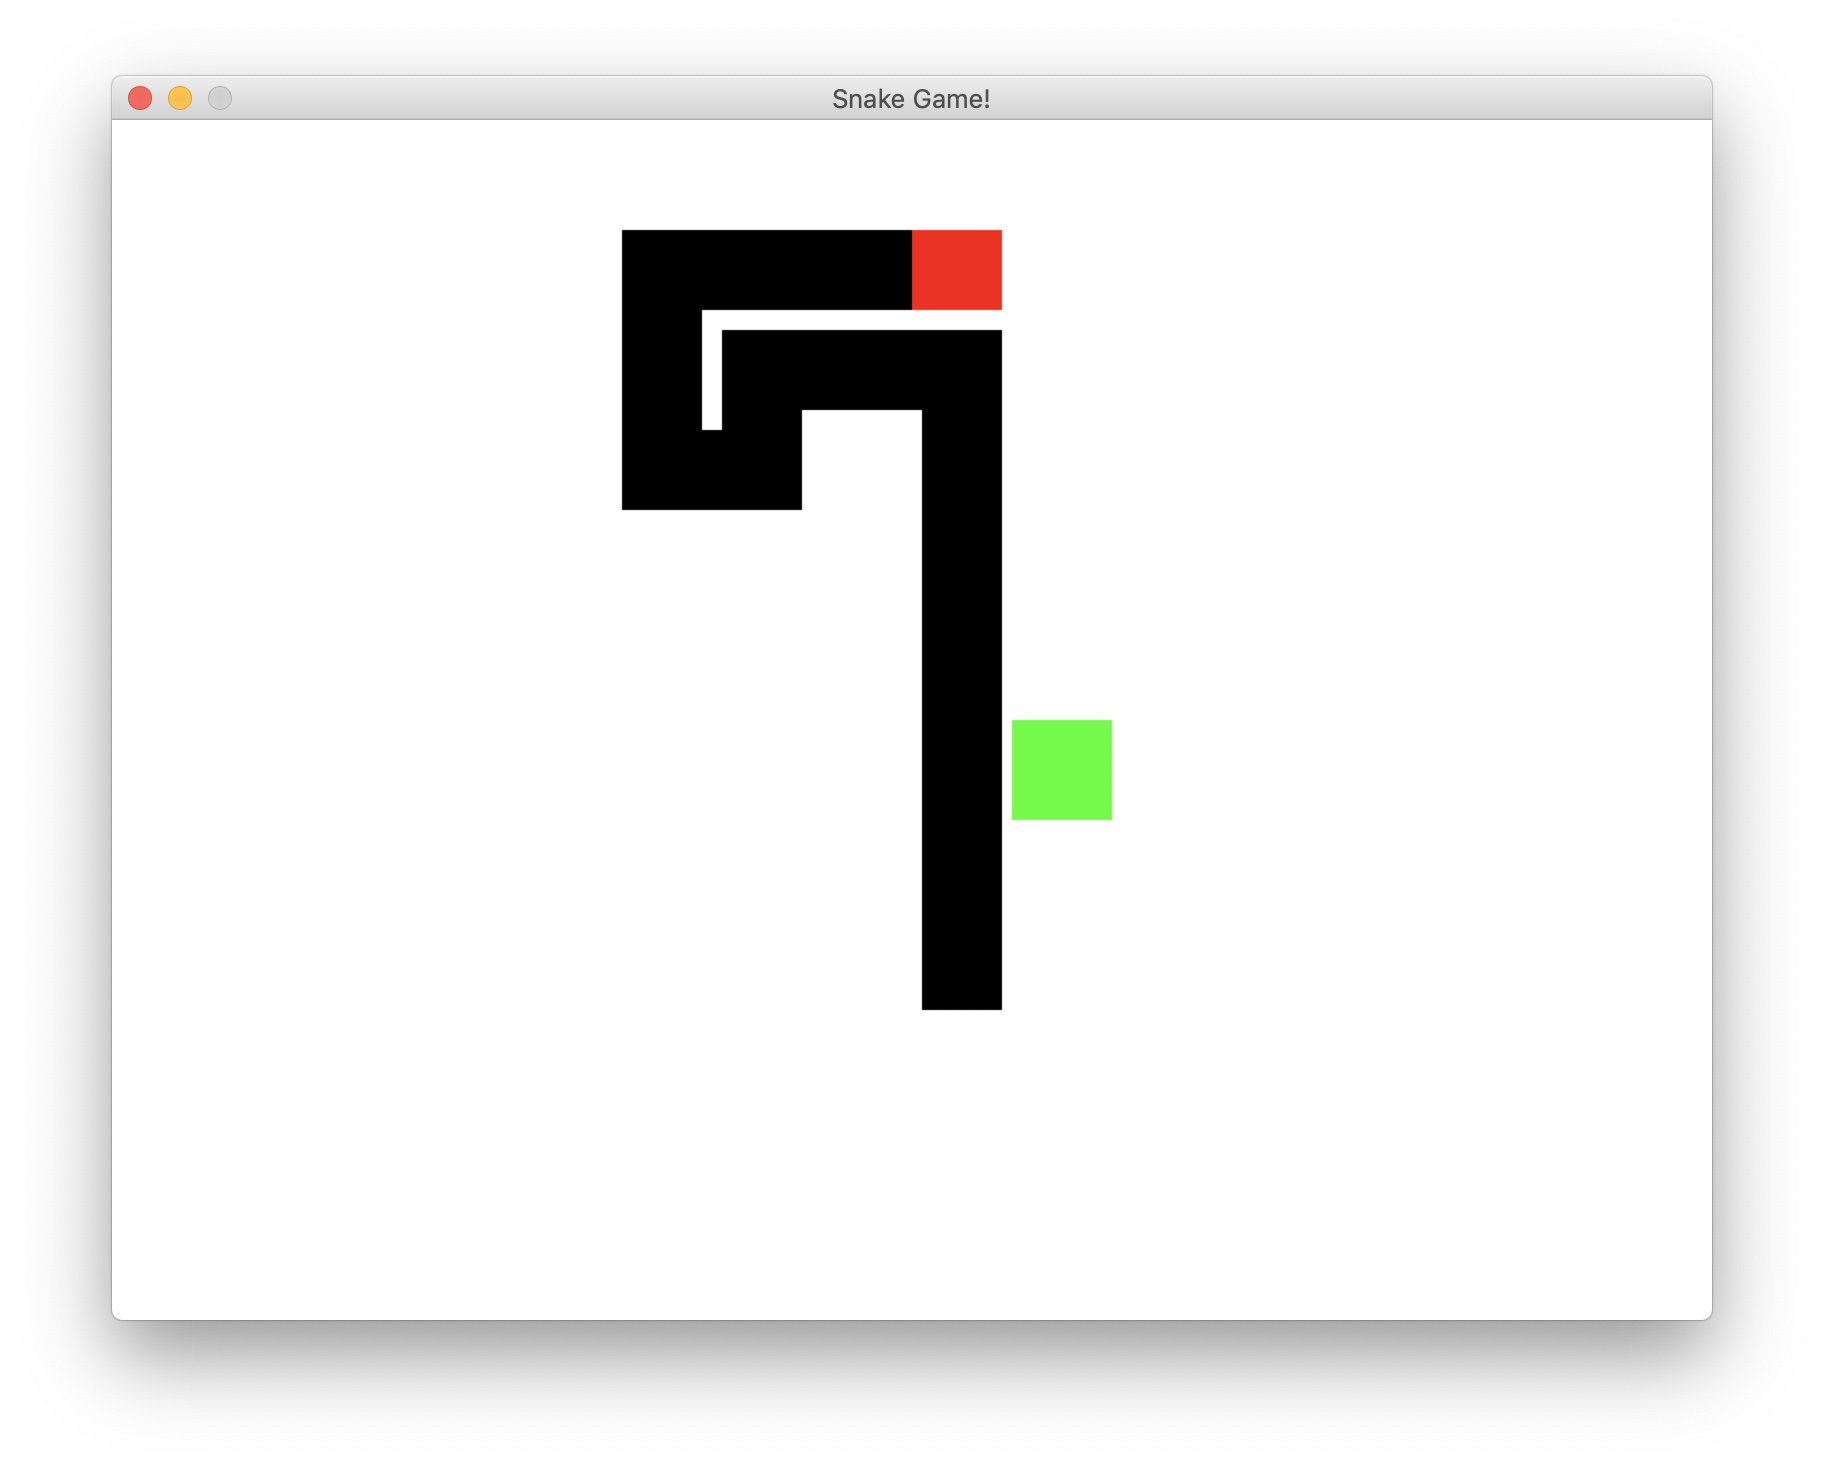
\includegraphics[scale=0.4]{assets/game.png}
    \caption{游戏界面截图\label{fig:game}} 
    \end{center} 
\end{figure} 

\subsection{自动寻路算法}\autoref{subsec:intro-route}
自动寻路算法为贪吃蛇赋予一定的智能,让其能正确地完成游戏。此处的``正确''有两层含义
\begin{itemize}
    \item 当贪吃蛇能触碰水果时,其应主动沿较优路接近水果
    \item 任何时候,当下一步行动可能造成贪吃蛇的死亡时,贪吃蛇应避免该行动
\end{itemize}
目前实现自动寻路的方法有很多,例如
\begin{enumerate} [label=(\alph*)]
    \item 朴素贪心算法
    \item 保守Hamilton回路算法
    \item 改良Hamilton回路算法
    \item 遗传算法
    \item 改良的贪心算法
\end{enumerate}
这些方法会在\autoref{sec:eval}作详细描述。其中本项目使用的是改良的贪心算法。\\

\emph{NOTE:本项目使用的改良贪心算法,可以证明其正确性。它的效率和准确度都是所有
算法中最高的。}
\section{项目闪光点}
\subsection{效果优良的寻路算法}
\subsection{无向图最长路近似算法}
\subsection{解耦的实现}
TODO:
\section{环境与运行}
\subsection{运行环境介绍}\label{subsec:env}
运行本项目代码需Python3.5及以上和Pygame组件库。一种参考的安装和运行方法
见\autoref{lst:install}。\\

在\autoref{lst:install}中,需要预安装python虚拟环境管理工具conda(并非必要),
并使用pip安装pygame组件库。在安装完毕后,使用cd命令进入code/目录,并直接运行main.py程序
即可。

\begin{figure}[!hbt]
\begin{itemize}
\item[] \begin{lstlisting}[style=myshell, label=lst:install, caption=安装运行环境的参考方法]
$ conda create --name game python=3.7 
$ pip install pygame
$ cd code/
$ python main.py
\end{lstlisting}
\end{itemize}
\end{figure}

\subsection{运行方法和使用方法}
\subsubsection{程序运行}
使用\autoref{subsec:env}介绍的方式(或其他等价方式)安装环境并运行main.py代码。
以下假设程序已正常运行。

\subsubsection{配置文件}
本游戏给予玩家很大的可配置性,许多参数都存放在配置文件(config.json)中。这里提供了一份默认的配置文件
(\autoref{lst:config}),但用户可以随意按需修改。\\

\emph{NOTE:在main.py文件的同一目录下,必须存在一份config.json文件,否则游戏因缺少参数
而无法运行}。\\

在配置文件中,window-width和window-height分别指定游戏窗口的大小。block-size指定
游戏中一个``块''的大小(贪吃蛇每次以块为单位移动)。块必须能整除window-width和window-height。
speed是游戏速度,决定贪吃蛇的移动间隔时间(秒)。auto指是否开启AI自动寻路。

\begin{figure}[!hbt]
\begin{itemize}
\item[] \begin{lstlisting}[style=mypython, label=lst:config, caption=config.json配置文件(默认)]
{
    "window-width": 800,
    "window-height": 600,
    "block-size": 50,
    "speed": 0.3,
    "auto": true
}
\end{lstlisting}
\end{itemize}
\end{figure}

\subsubsection{游戏键位}
使用W,S,A,D分别控制贪吃蛇向上、下、左、右运动。使用U和I控制游戏的速度,U加快游戏速度,
I减慢游戏速度。使用Q退出游戏。\\

(按下空格键以产生一份"output\_\emph{<hash>}.log"文件,用于debug)。

\section{代码文件介绍}
\subsection{主文件 main.py}
main.py调用了其他所有的文件,是玩家直接运行的程序。\\

该文件使用Snake类和Fruit类存储了地图信息,使用Pygame绘制了游戏窗口,
使用SnakeDrawer和FruitDrawer为不断变化的snake和fruit更新绘制图像。
同时,Pygame还负责监听键盘事件,响应玩家的操控。main.py还负责使用
延时来处理游戏速度。
\subsection{游戏类 snake.py 和 fruit.py}
Snake类和Fruit类分别定义在snake.py和fruit.py上。\\

Snake类存储了贪吃蛇的内部状态,例如所有蛇身所在的坐标(特别地,蛇头
看做第一段蛇身),蛇的当前方位等。Snake类暴露了若干接口,用于设置蛇的
当前走向、控制蛇向前一步,检验蛇是否处于非法状态等。\\

Fruit类存储了水果的内部状态,例如水果的当前坐标。Fruit类还实现了
generate函数,产生下一个水果的出现位置。由于水果不能出现在蛇身占用
的格子上,故Fruit的generate函数可能会被反复调用,直到得到的结果
符合游戏要求。

\subsection{寻路类 pather.py 和 solver.py}
pather.py是寻路类的主要模块,其中的类PathSolve是辅助工具,用于求出
蛇头距离水果的最短路,以及蛇头距离水果和蛇尾的最长路。\\

\emph{NOTE:无向图中的两点最长路是NP-Hard问题,但本项目使用了近似算法,
在小规模数据中取得了等价于精确解的效果。} \\

PathSolve使用了广度优先搜索算法得到最短路。可以容易地将其拓展为A-Star算法
获得更好的性能。但广搜的性能在此处已经足够好。同时,其采用了``最短路拓展''
的方法找到近似最长路,具体地说,它在最短路的基础上反复尝试将路拓展延长2个单位,
直到无法进行任何的拓展为止。更详细的介绍见\autoref{subsec:route}。\\

solver.py定义了GredySolver类。如名字所见,该类采用改良的贪心算法进行寻路。
当蛇可以轻易吃到水果时,蛇会优先以最短路走向水果,否则,蛇会以最长路
走向蛇尾。更详细的介绍见\autoref{subsec:route}。

\section{贪吃蛇游戏的具体实现}
\subsection{常亮定义}
在贪吃蛇项目中,定义以下的若干常量可以简化代码的书写,使得代码的可读性更好。
\begin{table}[!htb]
\caption{常量定义}\label{tab:const}
\begin{tabular}{@{} *5l @{}}
    \toprule
    \emph{常量名} & \emph{取值} &\emph{备注}&& \\
    \midrule
    % \ [a| ] & [b |] & c\\
    \ [UP | DOWN | LEFT | RIGHT]  & [0 | 1 | 2 | 3] & 他们同时可以作为列表的索引 \\
    \ [BLACK | WHITE | GREEN] & [(0, 0, 0) | (255, 255, 255) | (0, 255, 0)] & Pygame以RGB的形式表示颜色 \\
    \bottomrule
\hline
\end{tabular}
\end{table}

\subsection{Snake类的具体实现}
Snake类定义了一系列接口(\autoref{tab:snake-int})。它们大致可以分为返回状态的
接口和更新状态的接口。\\

返回状态的接口包括head, tail, direction, nextHead, valid, at等。\\

nextHead是必要的,这是因为如果蛇下一步前进时会触碰到水果,新的水果必须在同一时刻
出现在地图上。知道蛇头下一刻处于的位置是有好处的。\\

at用于判断地图上的某个方块是否被蛇身占用。在生成水果时会用到。水果必须生成在
不被蛇身占用的方块上。 \\

有副作用的函数包括next, eatFruit等。其中调用next后会使得蛇前进一个块。
Snake类中存储了蛇身的坐标以及蛇头方向。在调用next后,蛇头向前延伸一个单位,并把
延伸的块的坐标插入到蛇身的第一个元素(.insert(0, *))。还要把蛇身的最后一个元素
删除(.pop())。\\

eatFruit被调用后,蛇的内部状态会记录着当前吃到了一个水果(hasEat = True);在下一次next被调用时,
不再把蛇身的最后一个元素删除(相当于蛇身变长一个单位)。无论怎样,在调用next后都会把吃到水果的状态置空(hasEat = False)。\\

注意到许多函数是\emph{幂等}的。幂等的意思是,这些函数连续调用一次以上的效果和只调用一次
的结果是一样的。例如连续多次turn(RIGHT),或者多次调用getHead。幂等的性质可以给
编程带来极大的便捷。(此处留意,turn(RIGHT)的RIGHT指的是绝对的右方,而不是指相对于
蛇头的右方)。


\begin{table}[!htb]
\caption{贪吃蛇类的主要接口}\label{tab:snake-int}
\centering
\begin{tabular}{@{} *5l @{}}
    \toprule
\emph{成员函数} & \emph{参数} & \emph{返回值} & \emph{备注} & \\
    \midrule
    head & None & Tuple(Int, Int) & 返回蛇头的坐标  \\
    tail & None & Tuple(Int, Int) & 返回蛇尾的坐标 \\
    direction & None & Str(Const) & 返回当前蛇的方向 \\
    nextHead & None & Tuple(Int, Int) & 返回下一步蛇头将会处于的位置 \\
    next &  None & None & 让蛇前进一步 \\
    turn & direction :: Str & None & 接受方向作为参数,调整蛇的走向 \\
    eatFruit & None &  None & 设置蛇的状态为``吃了水果'' \\
    valid & None & Boolean & 返回蛇是否咬到自己的身体 \\
    at & Position :: Tuple(Int, Int) & Boolean & 接受x-y坐标,返回该位置是否在蛇身上
    \\
    \bottomrule
\hline
\end{tabular}
\end{table}

\subsection{Fruit类的具体实现}
由于fruit类的实现比较简单,故直接放上代码(\autoref{lst:fruit})。\\

\_\_init\_\_函数主要读取了config的信息,设置了width和height两个内部状态。\\

函数generate、where和内部状态last\_generate的设计是比较好的,我后续的许多代码都
得益于这个接口而得到改进。\\

首先generate函数显式地产生随机坐标,将随机坐标记录到last\_generate上,并返回。
fruit类会一直维护着最后一次产生的随机坐标。事实上,这个``最近一次的随机坐标对''恰好
就是游戏当前水果所在的地点。where函数返回
\begin{itemize}
    \item 如果last\_generate为空,则调用generate后,再返回last\_generate 
    \item 否则,直接返回last\_generate
\end{itemize}
这个设计使得用户可以安全地随时调用where函数,且确保where函数有合法的返回值。只有在
当前的状态过期时(水果被吃掉了),才有必要调用generate函数重新生成水果。\\

\emph{NOTE:最近一次产生的随机坐标,是当前游戏中水果的位置坐标}。



\begin{figure}[!hbt]
\begin{itemize}
\item[] \begin{lstlisting}[style=mypython, label=lst:fruit, caption=fruit类的具体实现]
class Fruit:
    def __init__(self, config):
        self.config = config
        # some code to get width from `config`
        self.width = ... 
        # some code to get height from `confgi`
        self.height = ... 
        self.last_generate = None
    def generate(self):
        x = random.randint(0, self.width - 1)
        y = random.randint(0, self.height - 1)
        self.last_generate = (x, y)
        return (x, y)
    def where(self):
        if self.last_generate is None:
            self.generate()
        return self.last_generate
\end{lstlisting}
\end{itemize}
\end{figure}

\subsection{Drawer和相关类的具体实现}
Drawer相关的类有三个。分别是Drawer, SnakeDrawer和FruitDrawer。其中Drawer类是
后两个类的基类。
\subsubsection{Drawer基类的实现}
Drawer类定义了两个基本函数(\autoref{lst:drawer}),分别是\_basic\_draw和
\_toLeftTop。下划线代表这两个成员函数是保护(protected)成员函数。\\

这里的实现牵扯到一些pygame的使用细节,但大体的思路是很明确的。本项目中,水果、蛇身
和蛇头都采用方块来表示。成员函数\_basic\_draw封装了画方块这一操作。\\

self.rect缓存了一个边长为blk的方块信息,其中blk是从配置文件中读取的内容。
在实际画出方块时,需要对self.rect作(以窗口左上角为原点的)平移操作。平移
时只需要修改self.rect对象中的topleft属性即可。该属性是个getter/setter语法糖,
在该属性被修改时,会触发self.rect修改其他相关属性(例如left, top等),以维持
方块的一致性。\\

\_basic\_draw函数首先对方块作平移,随后在Surface上画出这一方块。在函数\_basic\_draw中,
Surpface是对象screen。screen是代表整个窗口的Surface,由Drawer类被构造时传入。\\

\_toLeftTop接受坐标x和y,返回x行y列的方块的topleft值。
\begin{figure}[!hbt]
\begin{itemize}
\item[] \begin{lstlisting}[style=mypython, label=lst:drawer, caption=Drawer基类]
class Drawer():
    def __init__(self, screen, config):
        self.blk = int(config['block-size'])
        self.rect = pygame.Rect(0, 0, self.blk, self.blk)
        self.screen = screen
    def _basic_draw(self, x, y, color):
        self.rect.topleft = self._toLeftTop(x, y)
        pygame.draw.rect(self.screen, color, self.rect)
    def _toLeftTop(self, x, y):
        return (x * self.blk, y * self.blk)
\end{lstlisting}
\end{itemize}
\end{figure}

\subsubsection{SnakeDrawer}
SnakeDrawer的成员函数如\autoref{tab:snakedrawer-int}所示。\\

其中\_\_remove和\_\_draw函数调用了基类的函数\_basic\_draw。函数next是
有副作用的函数,它和Snake类的耦合度比较高。它的作用是,调用Snake函数的next方法,
让蛇向前行走一步,并\emph{仅仅}更新蛇头和蛇尾两个方块。这样的目的是加快程序的运行
效率。绘制图形和刷新窗口是非常费时的操作,加快程序运行方法有两个层面。
\begin{itemize}
    \item 尽可能减少窗口的刷新范围
    \item 尽可能较小窗口的刷新频率
\end{itemize}
SnakeDrawer和Snake类在next方法上强耦合,但能``减少窗口刷新范围''。 \\

SnakeDrawer类还有一个draw成员函数,它的作用是画出全部的蛇身。在整个游戏窗口
初始化时,这个函数会被调用。但随后,对snake的所有绘图都仅适用next函数。

\begin{table}[!htb]
\caption{SnakeDrawer的主要接口}\label{tab:snakedrawer-int}
\centering
\begin{tabular}{@{} *5l @{}}
    \toprule
\emph{成员函数} & \emph{参数} & \emph{返回值} & \emph{备注} & \\
    \midrule
    draw & None & None & 画出整条蛇的全部方块 \\
    next & None & None & \textbf{有副作用},调用蛇的next函数,更新蛇的图像 \\
    \_\_remove & Int, Int & None & 接受坐标,对该坐标的方块画上背景色 \\
    \_\_draw & Int, Int & None & 接受坐标,对该坐标的方块画上蛇身颜色 \\
    \bottomrule
\hline
\end{tabular}
\end{table}

\subsection{FruitDrawer}
FruitDrawer的定义如\autoref{lst:fruitdrawer}所示。\\

该实现比较简单,故直接附上源码。它仅提供了draw接口,它调用了Fruit的where成员函数,
画出水果的当前位置。
\begin{figure}[!hbt]
\begin{itemize}
\item[] \begin{lstlisting}[style=mypython, label=lst:fruitdrawer, caption=FruitDrawer定义]
class FruitDrawer(Drawer):
    def __init__(self, screen, config, fruit):
        Drawer.__init__(self, screen, config)
        self.fruit = fruit
        self.width = int(int(config['window-width']) / config['block-size'])
        self.height = int(int(config['window-height']) / config['block-size'])
    def draw(self):
        x, y = self.fruit.where()
        self._basic_draw(x, y, GREEN)
\end{lstlisting}
\end{itemize}
\end{figure}

\section{自动寻路算法的具体实现}\label{subsec:route}
本节介绍自动寻路算法的具体实现。它基于几个简单的搜索算法,在整体上使用贪心的思想。
\subsection{寻路算法介绍}
常用的寻路算法有许多种,以下详细见介绍。
\subsubsection{朴素贪心算法}
朴素贪心算法采用最朴素的贪心法。在每一步中,直接搜索从蛇头到水果的最短路,并按该
条路线前往水果。\\

该方法的优点是易于实现,思路简洁。但它的缺点也很明显。在贪吃蛇游戏中,局部最优解
一般都不为全局最优解(且往往相差很远)。这不满足我们在\autoref{subsec:intro-route}中提出的
``任意时刻贪吃蛇应避免死亡''的要求。\\

如\autoref{fig:naive-greedy}所示。如果贪吃蛇按箭头方向根据最短路吃到了水果,
它会因所有的出口都被堵住而游戏失败。 \\

很快可以看到,在朴素贪心算法的基础上添加``无向图最长路近似算法'',结合起来得到的改良版本可以
获得很好的性能。见\autoref{subsec:refine-greedy}。

\begin{figure}[!hbt]
    \begin{center}
    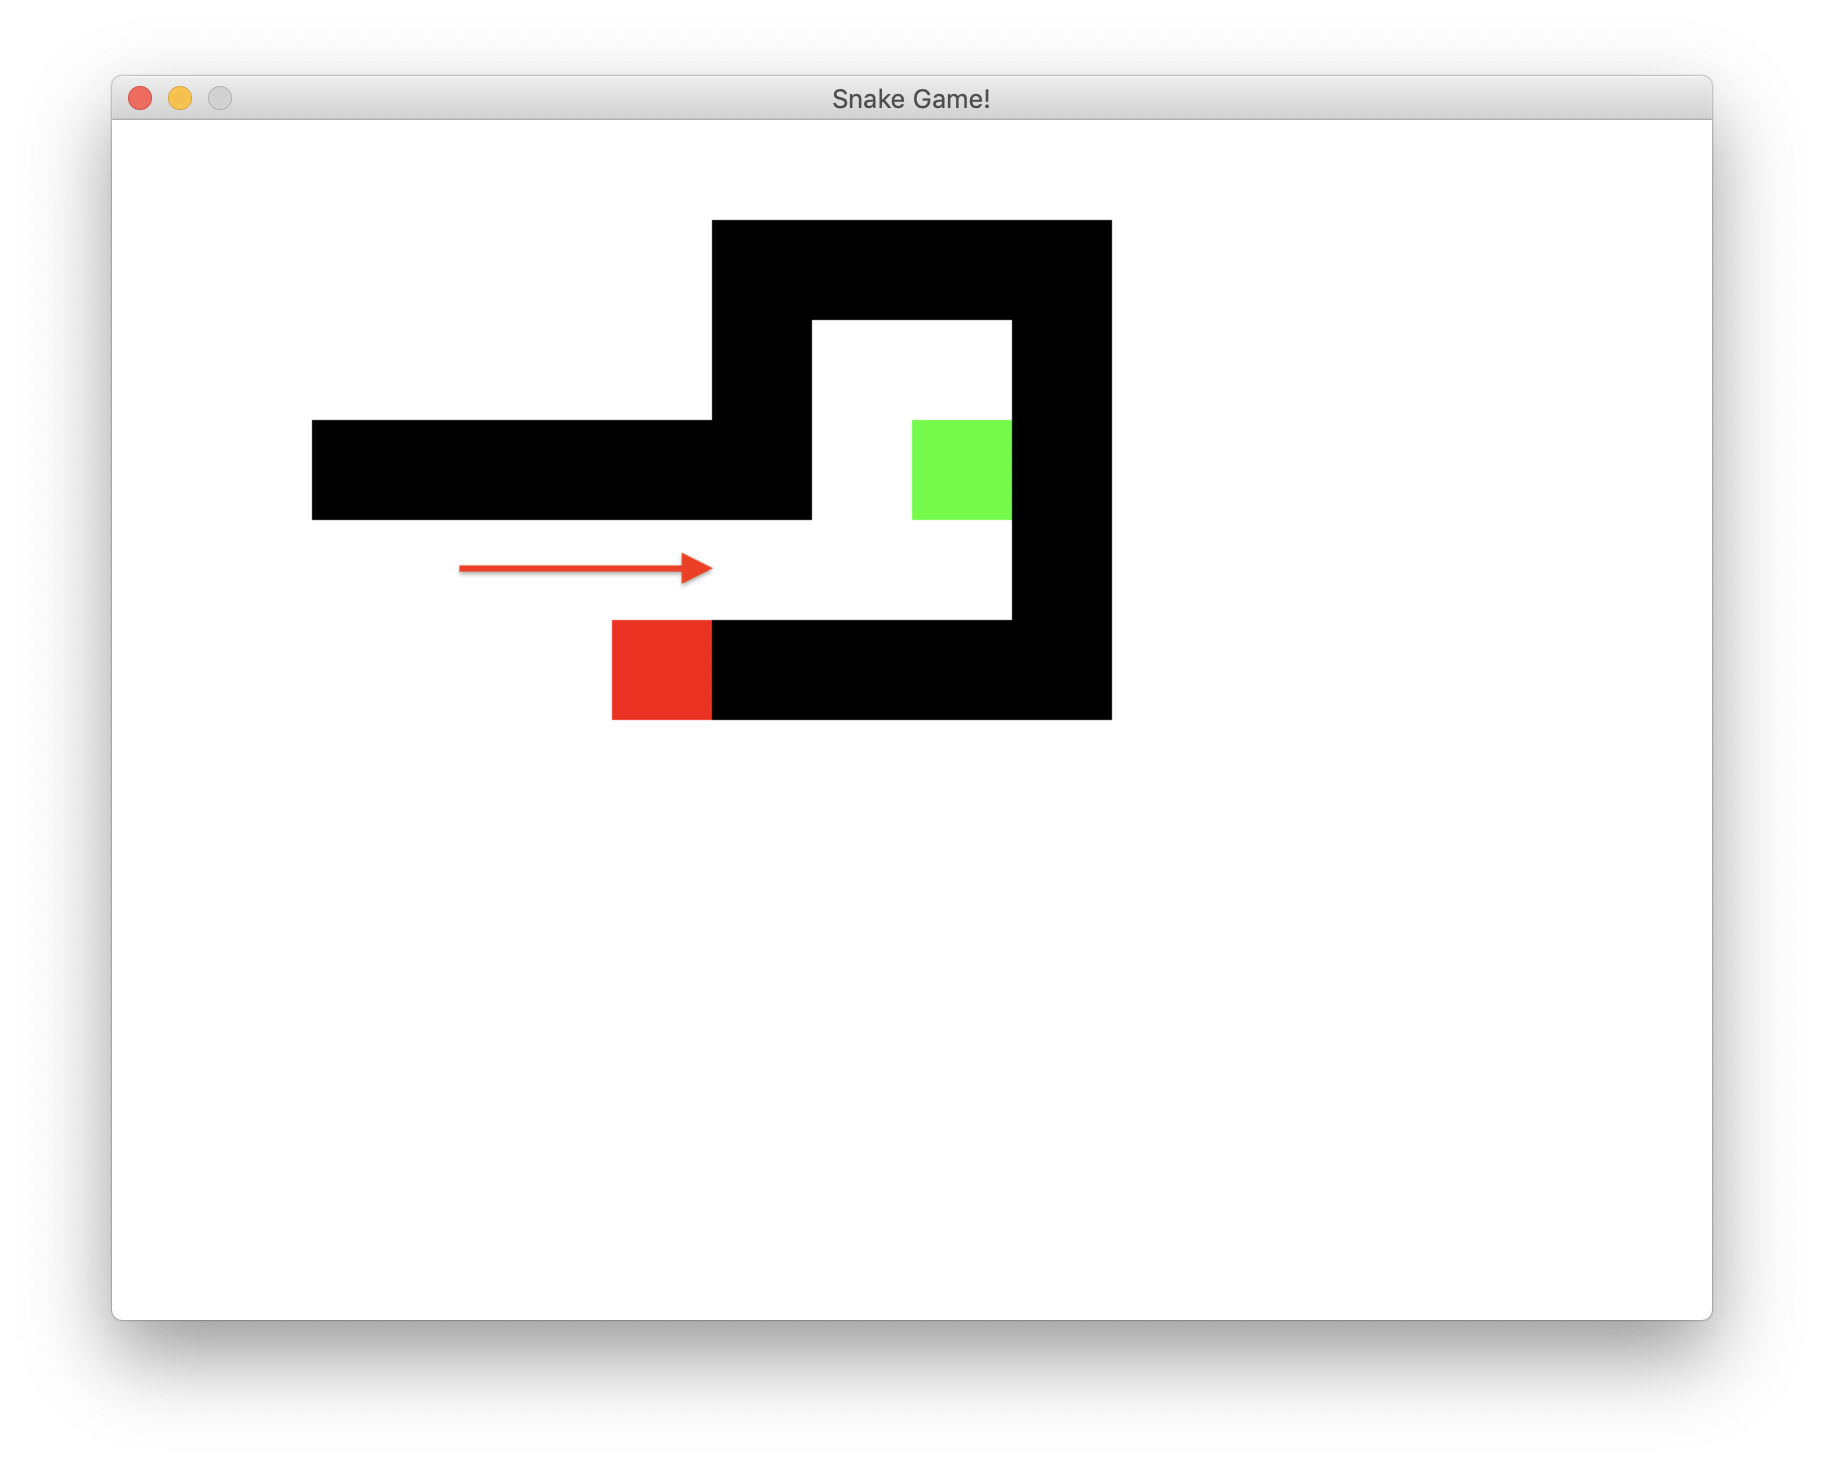
\includegraphics[scale=0.3]{assets/naive-greedy.png}
    \caption{朴素算法面临的困境\label{fig:naive-greedy}} 
    \end{center} 
\end{figure} 

\subsubsection{保守的Hamilton回路算法}
朴素Hamilton回路算法的思路很简单。其尝试在地图上构造一条哈密顿回路,然后永远按照该回路
在地图上无限循环地走(\autoref{fig:naive-hamilton})。显然这个算法是绝对正确的,而且贪吃蛇绝对不会死亡。但这却不满足
\autoref{subsec:intro-route}提出的``沿较优路前往水果''这个目标。\\

除此之外,这个算法还有一个隐含的要求,就是地图需要包含一条哈密顿回路。事实上这点是无法确保
的。对于不存在哈密顿回路的图,这个算法可能会失效。

\begin{figure}[!hbt]
    \begin{center}
    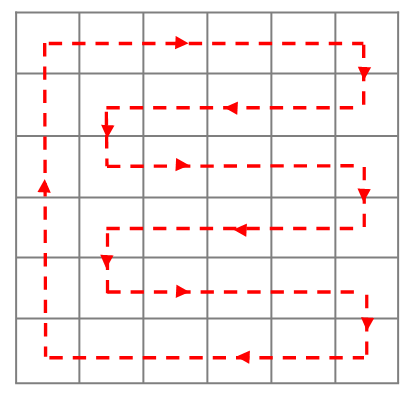
\includegraphics[scale=0.5]{assets/naive-hamilton}
    \caption{朴素Hamilton回路法介绍\label{fig:naive-hamilton}} 
    \end{center} 
\end{figure} 

\subsubsection{随机神经网络算法}
随机神经网络的方法是,使用纯随机(而非梯度下降)的方式优化参数。评价神经网络的
标准也不再是交叉熵或准确度,而是``贪吃蛇每局游戏的平均长度''。\\

具体来说,首先随机创建n个神经网络。每个神经网络的参数均来自独立的随机分布。神经网络
的输入是各种提前选定的属性,例如``蛇头距离水果的距离'', ``蛇头左侧是否有障碍''等等。
神经网络的输出是超参数,在整个模型训练中不变。神经网络的输出维度是3,分别表示``直行''、
``左转''和``右转''的自信度。\\

使用这n个随机创建的神经网络玩贪吃蛇游戏,记录他们的平均蛇长。取出效果最好的m个神经
网络(m一般比较小)。这为一轮训练。在这m个神经网络的基础上,加入随机的偏差,再次
产生n个随机的神经网络。如此重复,直到最后的神经网络能取得比较好的效果。\\

但这个算法有很大的缺点。例如
\begin{itemize}
    \item 需要人工选定输入的特征。难以选择合适的输入特征
    \item 效果较差。目前大部分基于神经网络的算法都难以在贪吃蛇游戏中取得比较好的效果
\end{itemize}
\begin{figure}[!hbt]
    \begin{center}
    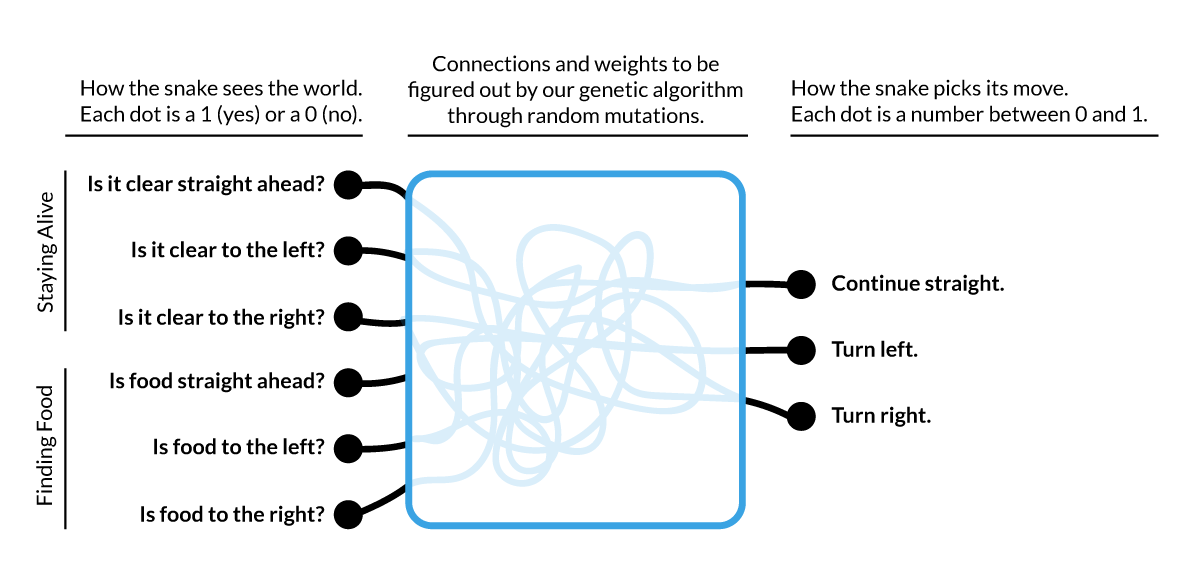
\includegraphics[scale=0.3]{assets/random-network.png}
    \caption{随机神经网络算法示意图\label{fig:random-network}} 
    \end{center} 
\end{figure} 

\subsubsection{改良的贪心算法}\label{subsec:refine-greedy}
改良的贪心算法是本项目选择实现的算法,可以证明它不会使得贪吃蛇游戏失败,且
在大部分情况下沿最短路前往水果。它的主要思路如下。\\


首先搜索一条蛇头到水果的最短路。然后假设贪吃蛇按照该最短路到达了水果。在此基础上,
检查蛇头是否有路径到达``蛇尾''。如果能到达蛇尾,说明蛇一定存在一个策略保证存活
(称此状态为安全状态)。如果不能,则说明蛇在吃了水果后的处境可能会``危险'', 
于是拒绝这个决策,选择在周围游荡,以``拖延时间''。

\subsection{改良贪心算法的具体实现}
\subsubsection{流程和正确性证明}
改良贪心算法的具体流程如下。为了寻找蛇$S_1$的最佳方向$D$
\begin{enumerate}[label=(\alph*)]
    \item 构造从蛇$S_1$到水果的最短路$P_1$。如果$P_1$存在,则执行(b)。否则执行(d)
    \item 构造一条虚拟的蛇$S_2 \gets S_1$,让$S_2$前进并吃到水果
    \item 构造蛇$P_2$从蛇头到蛇尾的最长路$P_2$。如果$P_2$存在,那么$D$就是$P_1$的第一个方向。否则,执行(d)
    \item 计算蛇$S_1$从蛇头到蛇尾的最长路$P_3$。如果$P_3$存在,那么$D$就是$P_3$的第一个方向。否则,执行(e)
    \item (worst case)$D$为远离水果的那个方向。
\end{enumerate}
对这个流程的相关解释如下。\\

在计算从蛇头到水果的最短路后,还要判断蛇$S_2$到其蛇尾是否具有最长路。这里要注意\\

\emph{NOTE:无向图的最长路算法是NP-Hard问题,此处使用了近似算法。在算法分析时,
最坏情况可能退化到最短路。}\\

若蛇$S_2$到蛇尾有最长路,可以得出蛇$S_2$到蛇尾必有路(显然)。可知,这样的走法是安全的,
这是因为\\

\emph{LEMMA: 当存在一条蛇头到蛇尾的路径时,贪吃蛇必不死。}\\

该引理是整个算法乃至整个项目最重要的一个理论基础。其奠定了改良贪心算法的准确性。\\

要论证这个引理很简单。首先,蛇头是不可能``追上''蛇尾的,这是因为每当蛇头往前前进一步,蛇尾也会向前
收缩一步。贪吃蛇只需要保证一刻不停地追逐蛇尾,就能保证必定不死。\\

于是贪吃蛇存在一种策略:
\begin{itemize}
    \item 贪吃蛇按照从蛇头到蛇尾的路前进
\end{itemize}
该策略可以保证贪吃蛇必定不死。

这就证明了上述引理的正确性。这同时解释了步骤(c)的用意:保证蛇不死。\\

在不那么好的场景下,有可能出现以下的局面
\begin{itemize}
    \item 蛇$S_1$不存在蛇头到水果的最短路$P_1$(步骤a的错误分支)
    \item 蛇$S_1$不存在从蛇头到蛇尾的最长路$P_3$(步骤d的错误分支)
\end{itemize}
当$P_1$不存在,说明了目前无法短时间内到达水果的位置。那蛇就应该尽可能地``绕远路'',
争取拖延更多的时间。同时绕远路也应该绕得安全,那么这个远路就应该是从蛇头到蛇尾的远路。
这就是(a)的错误分支跳转到(d)的解释。\\

若$S_1$不存在从蛇头到蛇尾的最长路,说明蛇在最坏情况下很可能已经进入了困境。算法中步骤(e)的
方法是向原理水果的方向运动。这是最坏情况下的无奈之举。\\

\emph{NOTE:从蛇头到蛇尾的最长路必定存在。这是因为(a)在游戏开始时,存在从蛇头到蛇尾
的最长路,且(b)在游戏的每次``状态转移''时都保证蛇头到蛇尾的最长路存在。故实际上上一情况
是不可能出现的。}

\subsection{最长路算法}
\subsubsection{算法思路}
最长路算法的基本步骤如下(\autoref{fig:build-longest})
\begin{itemize}
    \item 找到一条最短路
    \item 尝试拓展最短路,直到无法拓展为止
\end{itemize}
具体地说,在最短路p上定位相邻的两个结点。对于这每组相邻的结点,尝试将
他们从两个结点拓展到四个结点。例如相邻的结点A和B中,A向左走一步可以到达B([Left])。
拓展时,尝试拓展A到B的路[Down, Left, Up]。对称地,也可拓展为[Up, Left, Down]。\\

尝试画一下图显然得到,每次拓展都是把相邻的2个结点拓展成4个结点(类似于田字)。\\

这个拓展算法显然不是精确解,但在绝大部分情况下却能取得几乎最优的效果。\\


\autoref{fig:lp}的一系列图片是贪吃蛇沿着蛇头到蛇尾的最长路行进的示意图。
图左一是贪吃蛇的初始状态。红方块是蛇头,贪吃蛇(蜷缩)在一团。\\

在图左二中,贪吃蛇很聪明地旋转着绕远路,同时留下一条空隙,给予自己回过头来
回到蛇尾的机会。\\

左图三中,贪吃蛇绕远路达到了右边界,准备返回。\\

右图二中,贪吃蛇沿着左图一留下的``空隙''返回。逐步接近蛇尾。右图一中,
贪吃蛇最终到达了蛇尾。\\

\emph{这个最长路几乎是最优解,因为它的路径覆了整个地图,除了右上方的
一个方块。}
\begin{figure}[!hbt]
    \begin{center}
    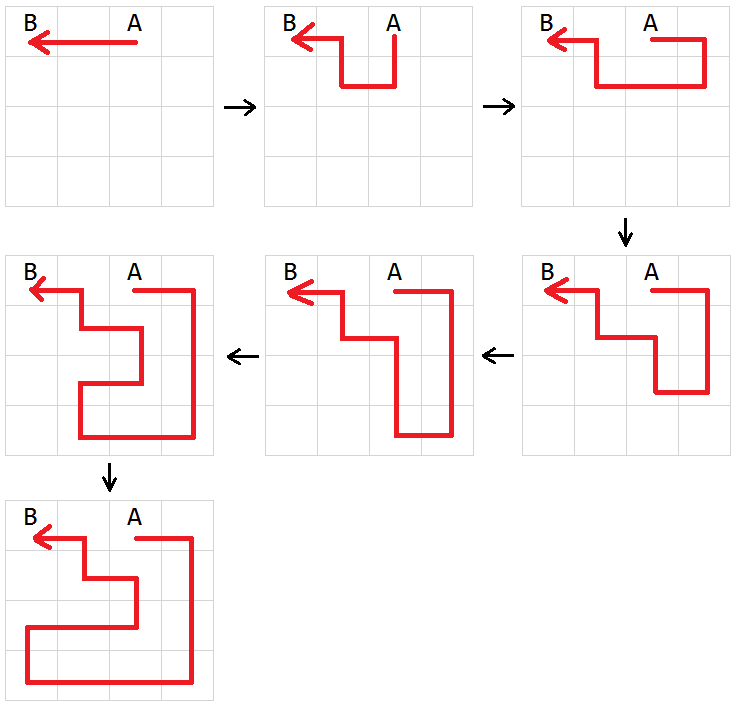
\includegraphics[scale=0.4]{assets/build-longest.png}
    \caption{最长路算法拓展示意图\label{fig:build-longest}} 
    \end{center} 
\end{figure} 

\begin{figure}[!hbt]
\begin{minipage}{0.19\textwidth}
    \centering
    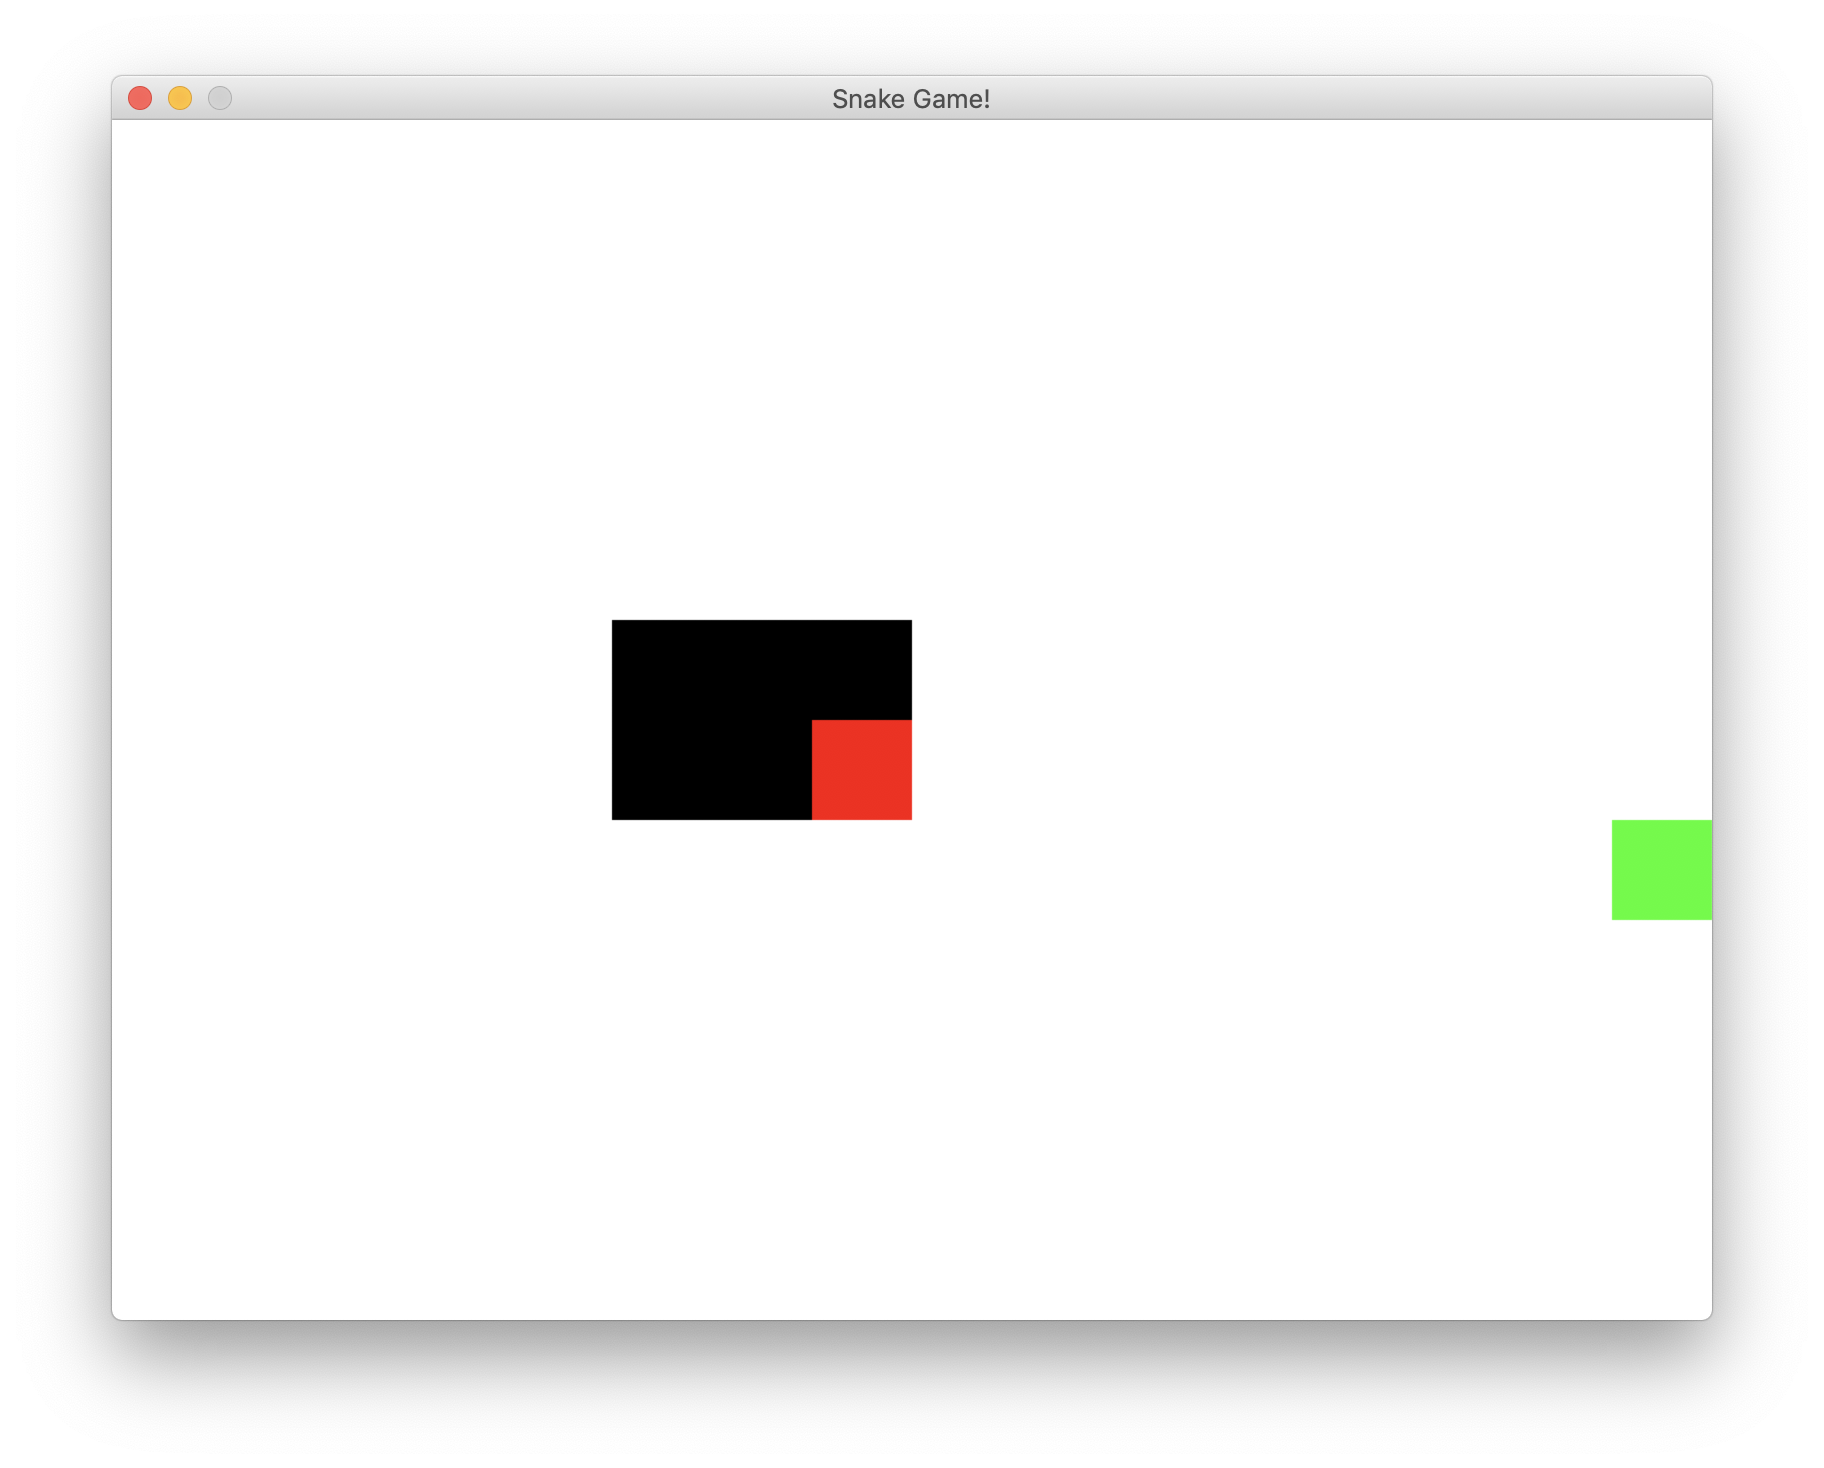
\includegraphics[width=\linewidth]{assets/lp1.png}
% \caption{caption} \label{fig:label}
\end{minipage}\hfill
\begin{minipage}{0.19\textwidth}
    \centering
    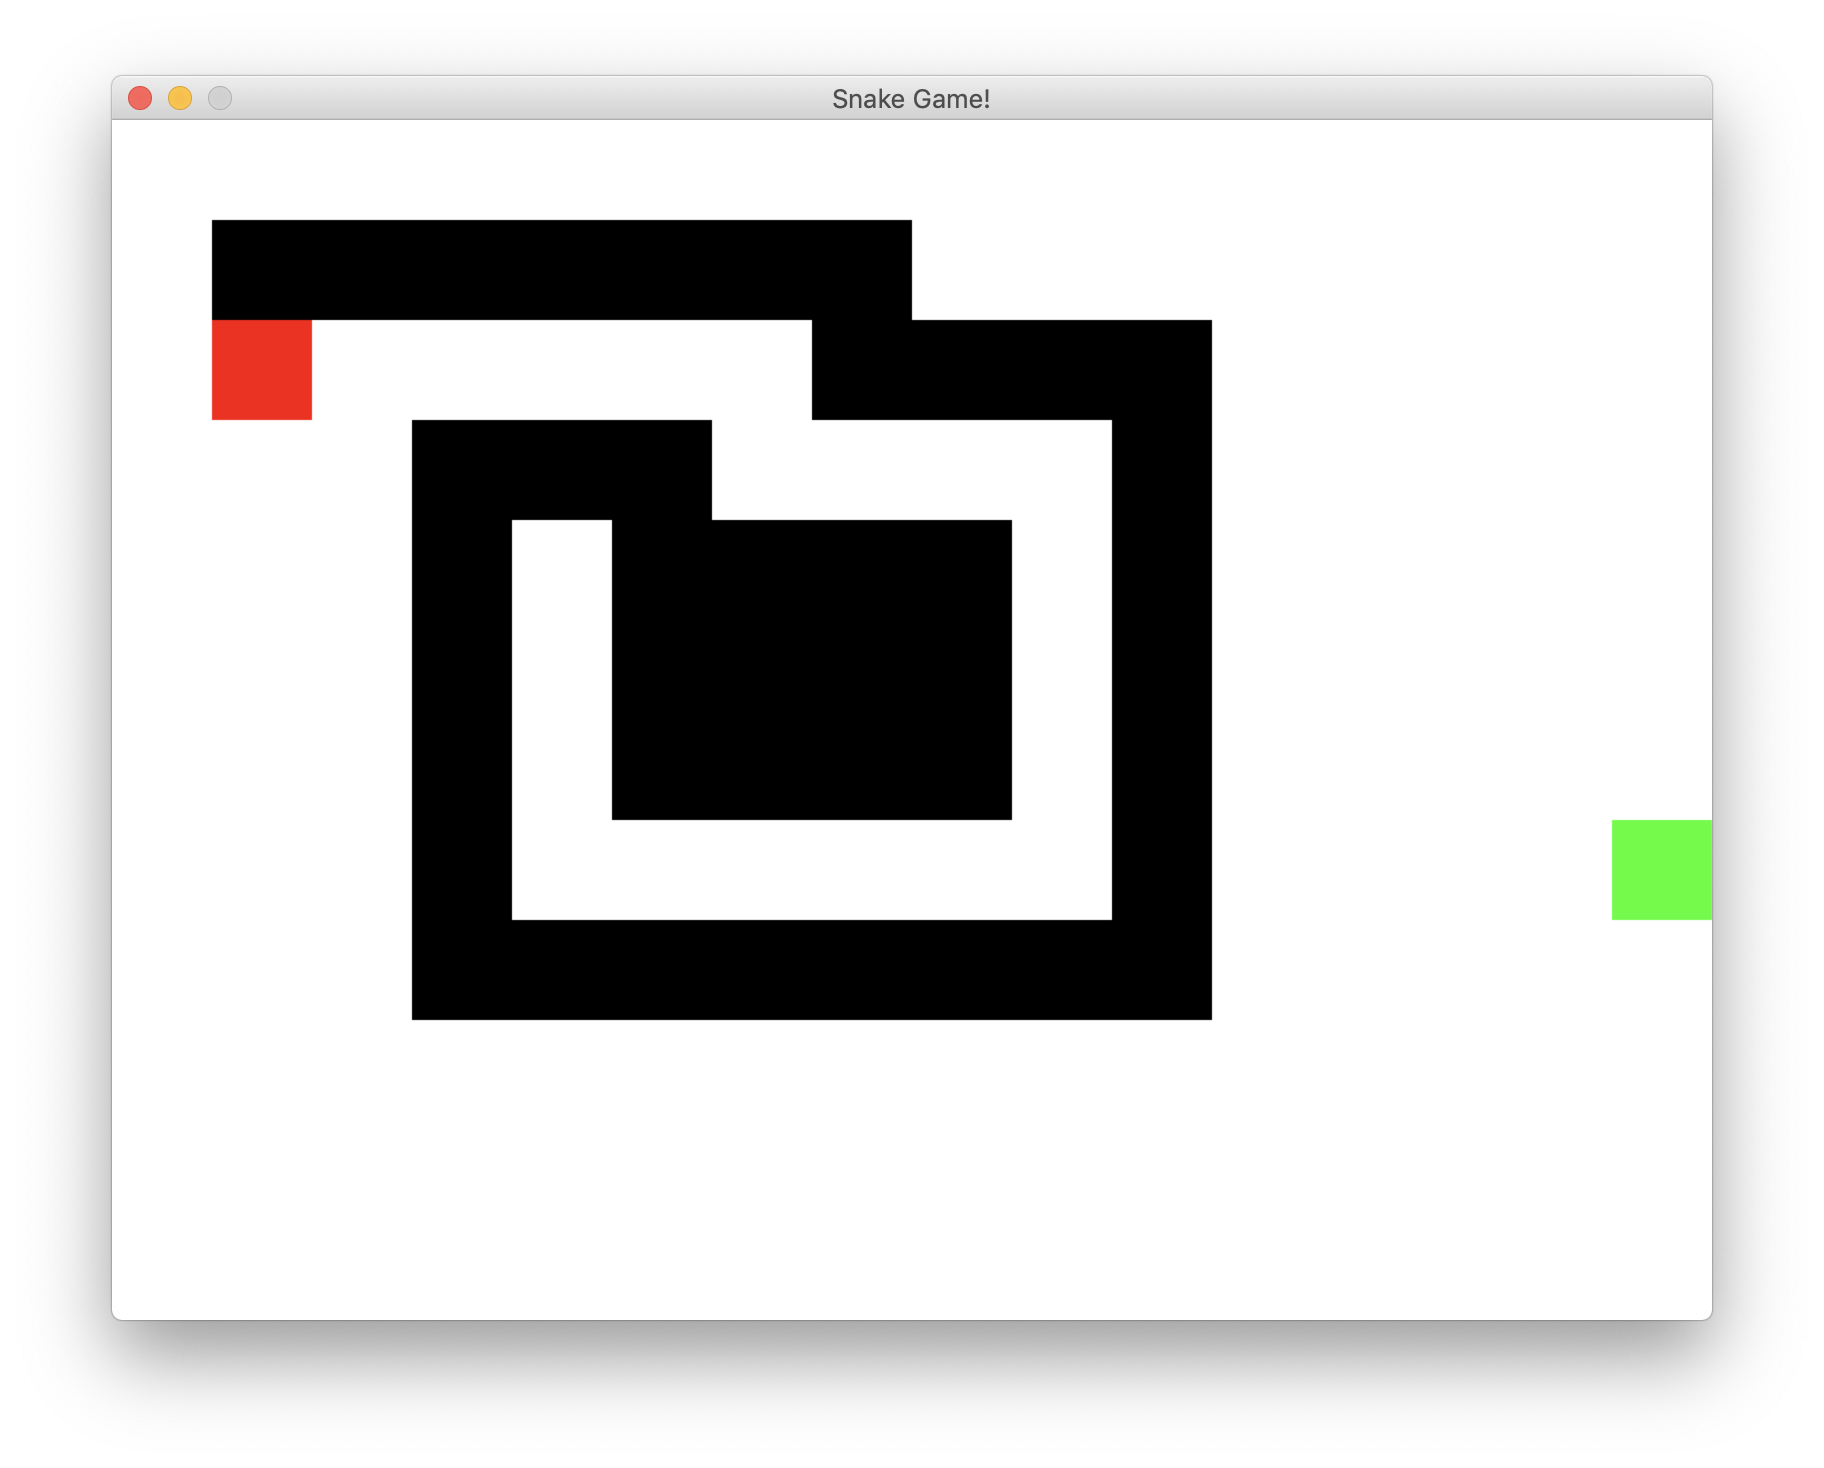
\includegraphics[width=\linewidth]{assets/lp2.png}
% \caption{caption} \label{fig:label}
\end{minipage}
\begin{minipage}{0.19\textwidth}
    \centering
    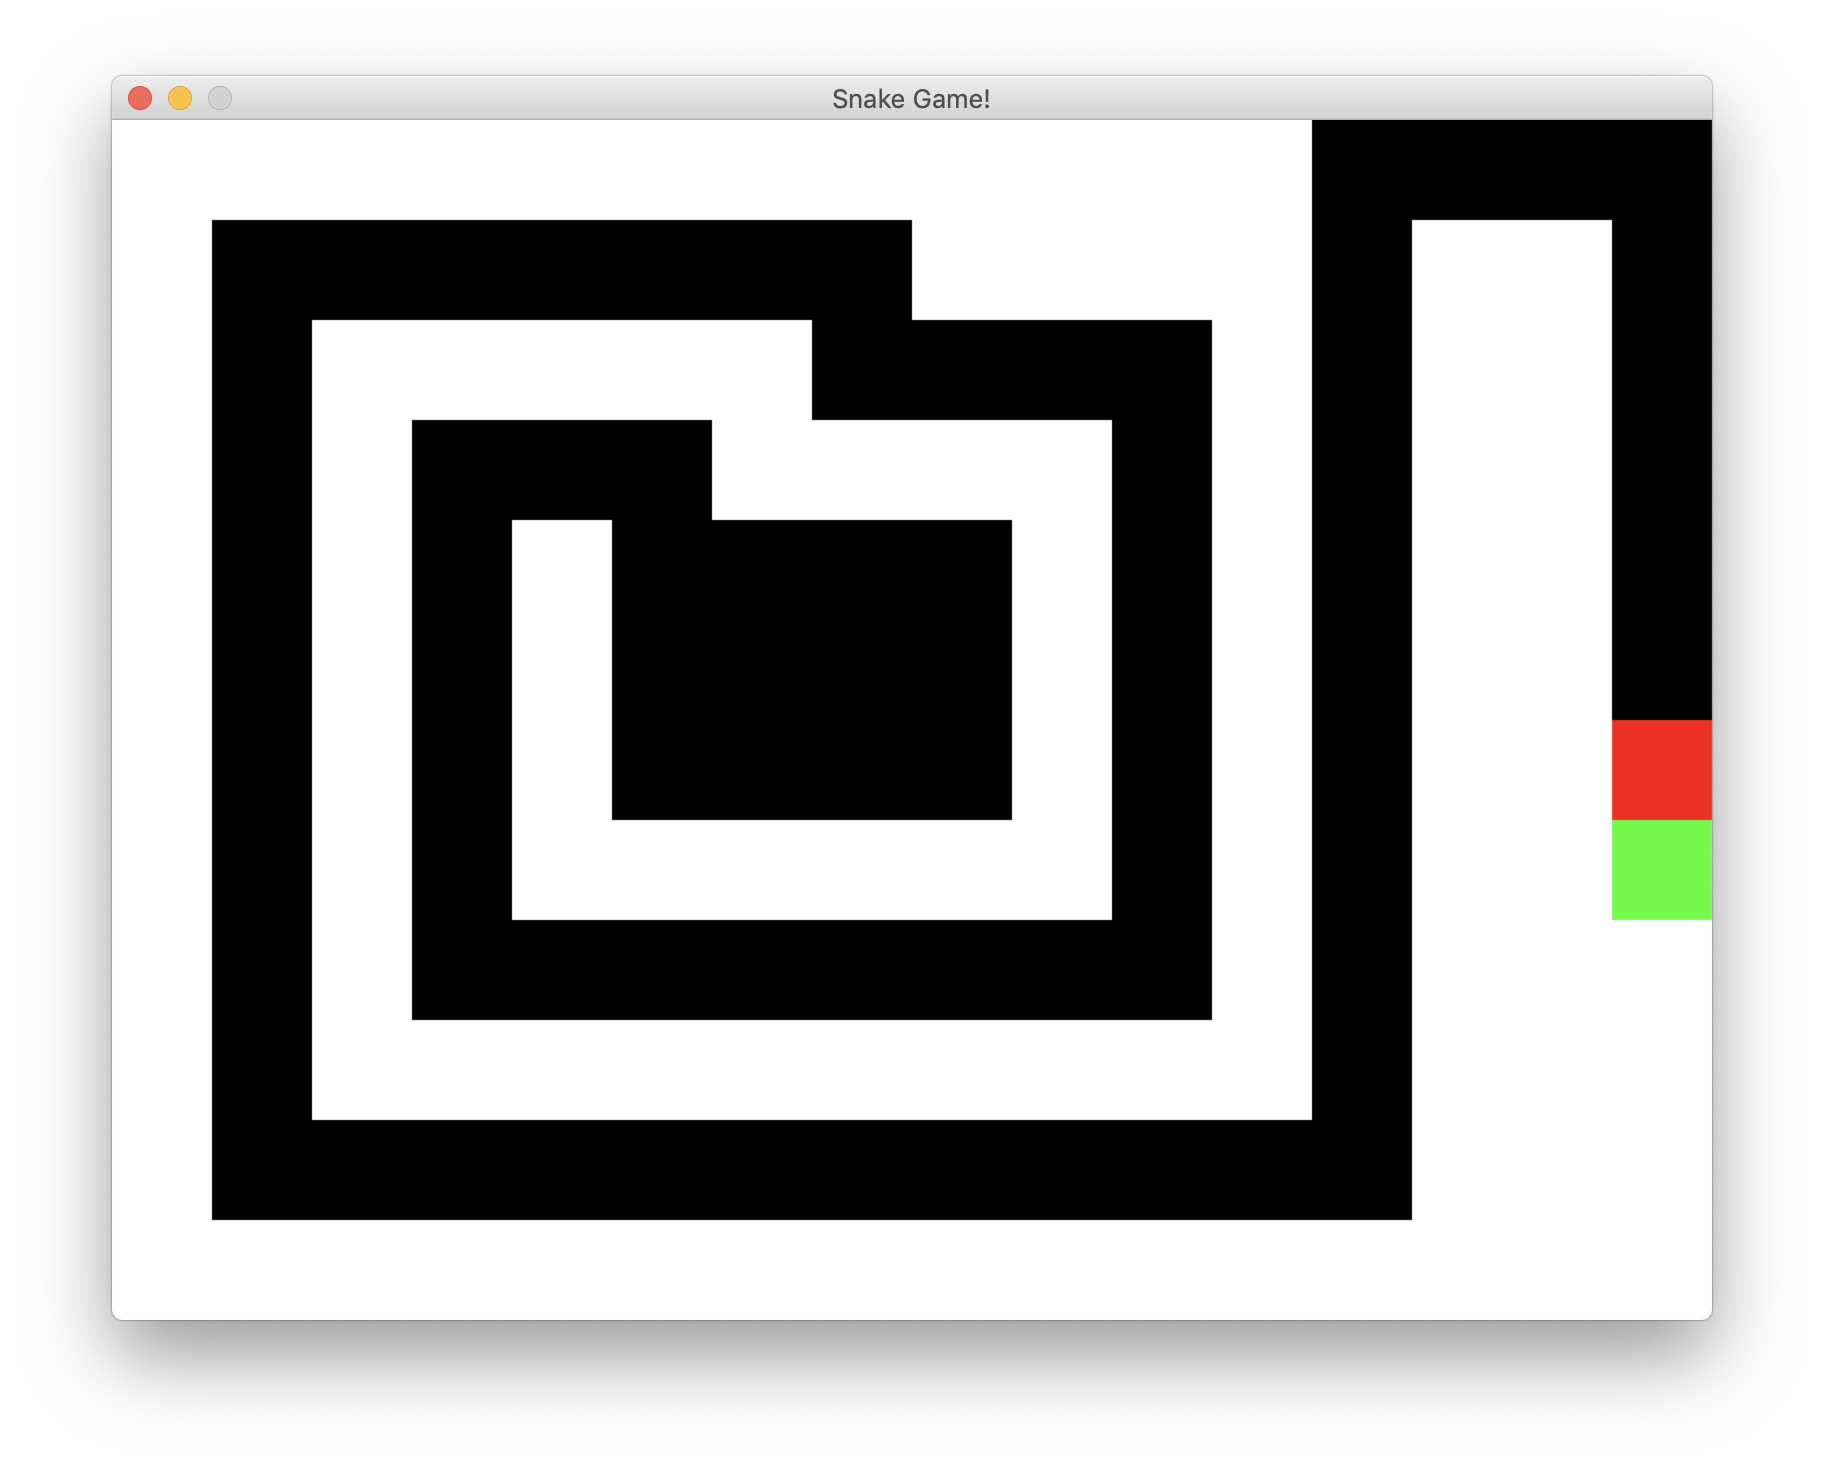
\includegraphics[width=\linewidth]{assets/lp3.png}
% \caption{caption} \label{fig:label}
\end{minipage}
\begin{minipage}{0.19\textwidth}
    \centering
    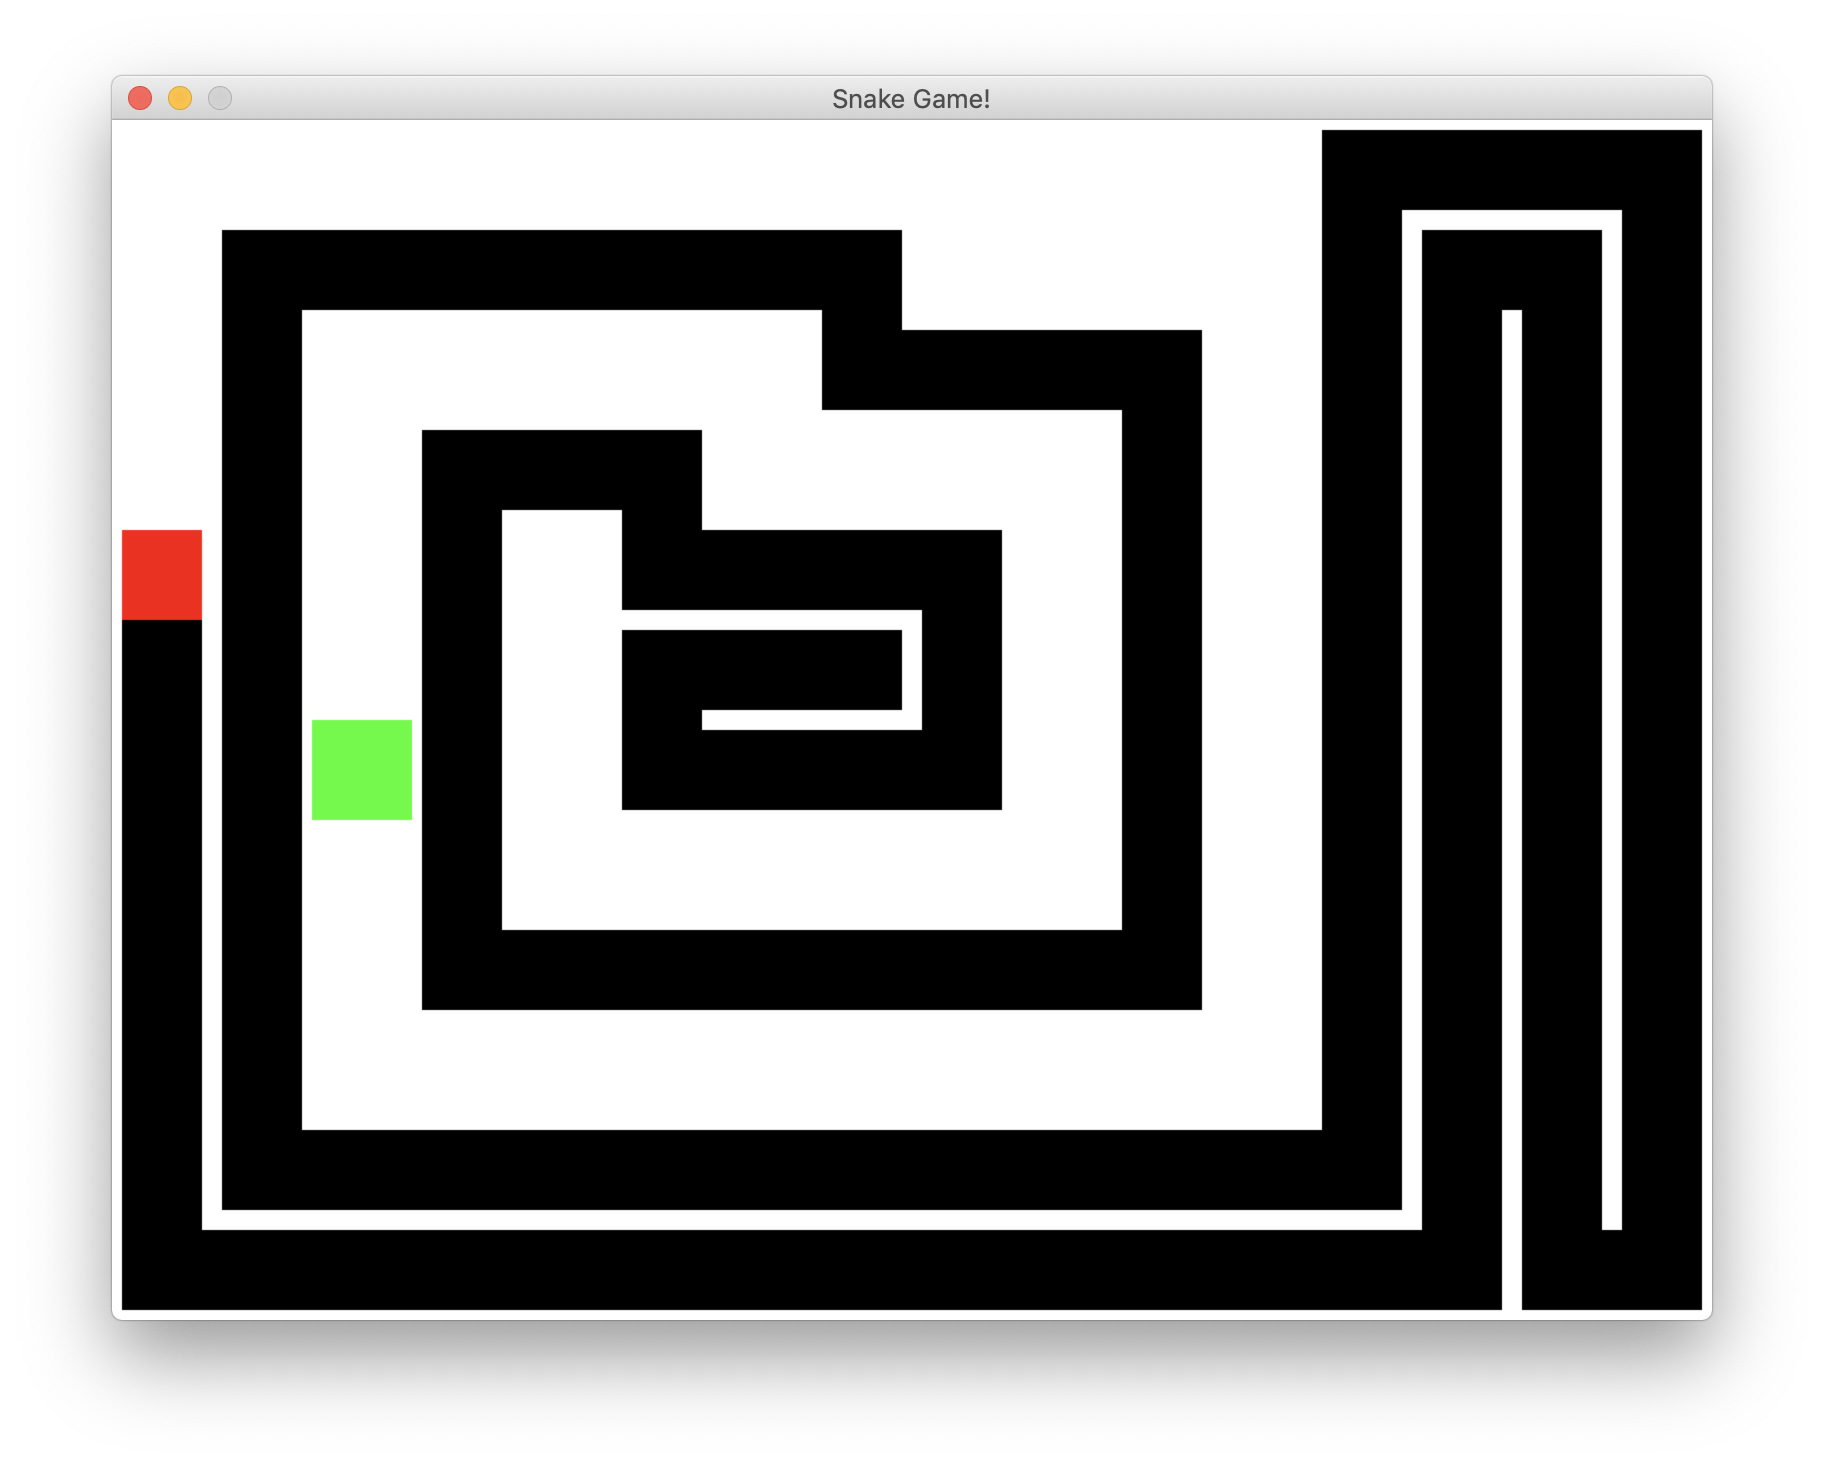
\includegraphics[width=\linewidth]{assets/lp4.png}
% \caption{caption} \label{fig:label}
\end{minipage}
\begin{minipage}{0.19\textwidth}
    \centering
    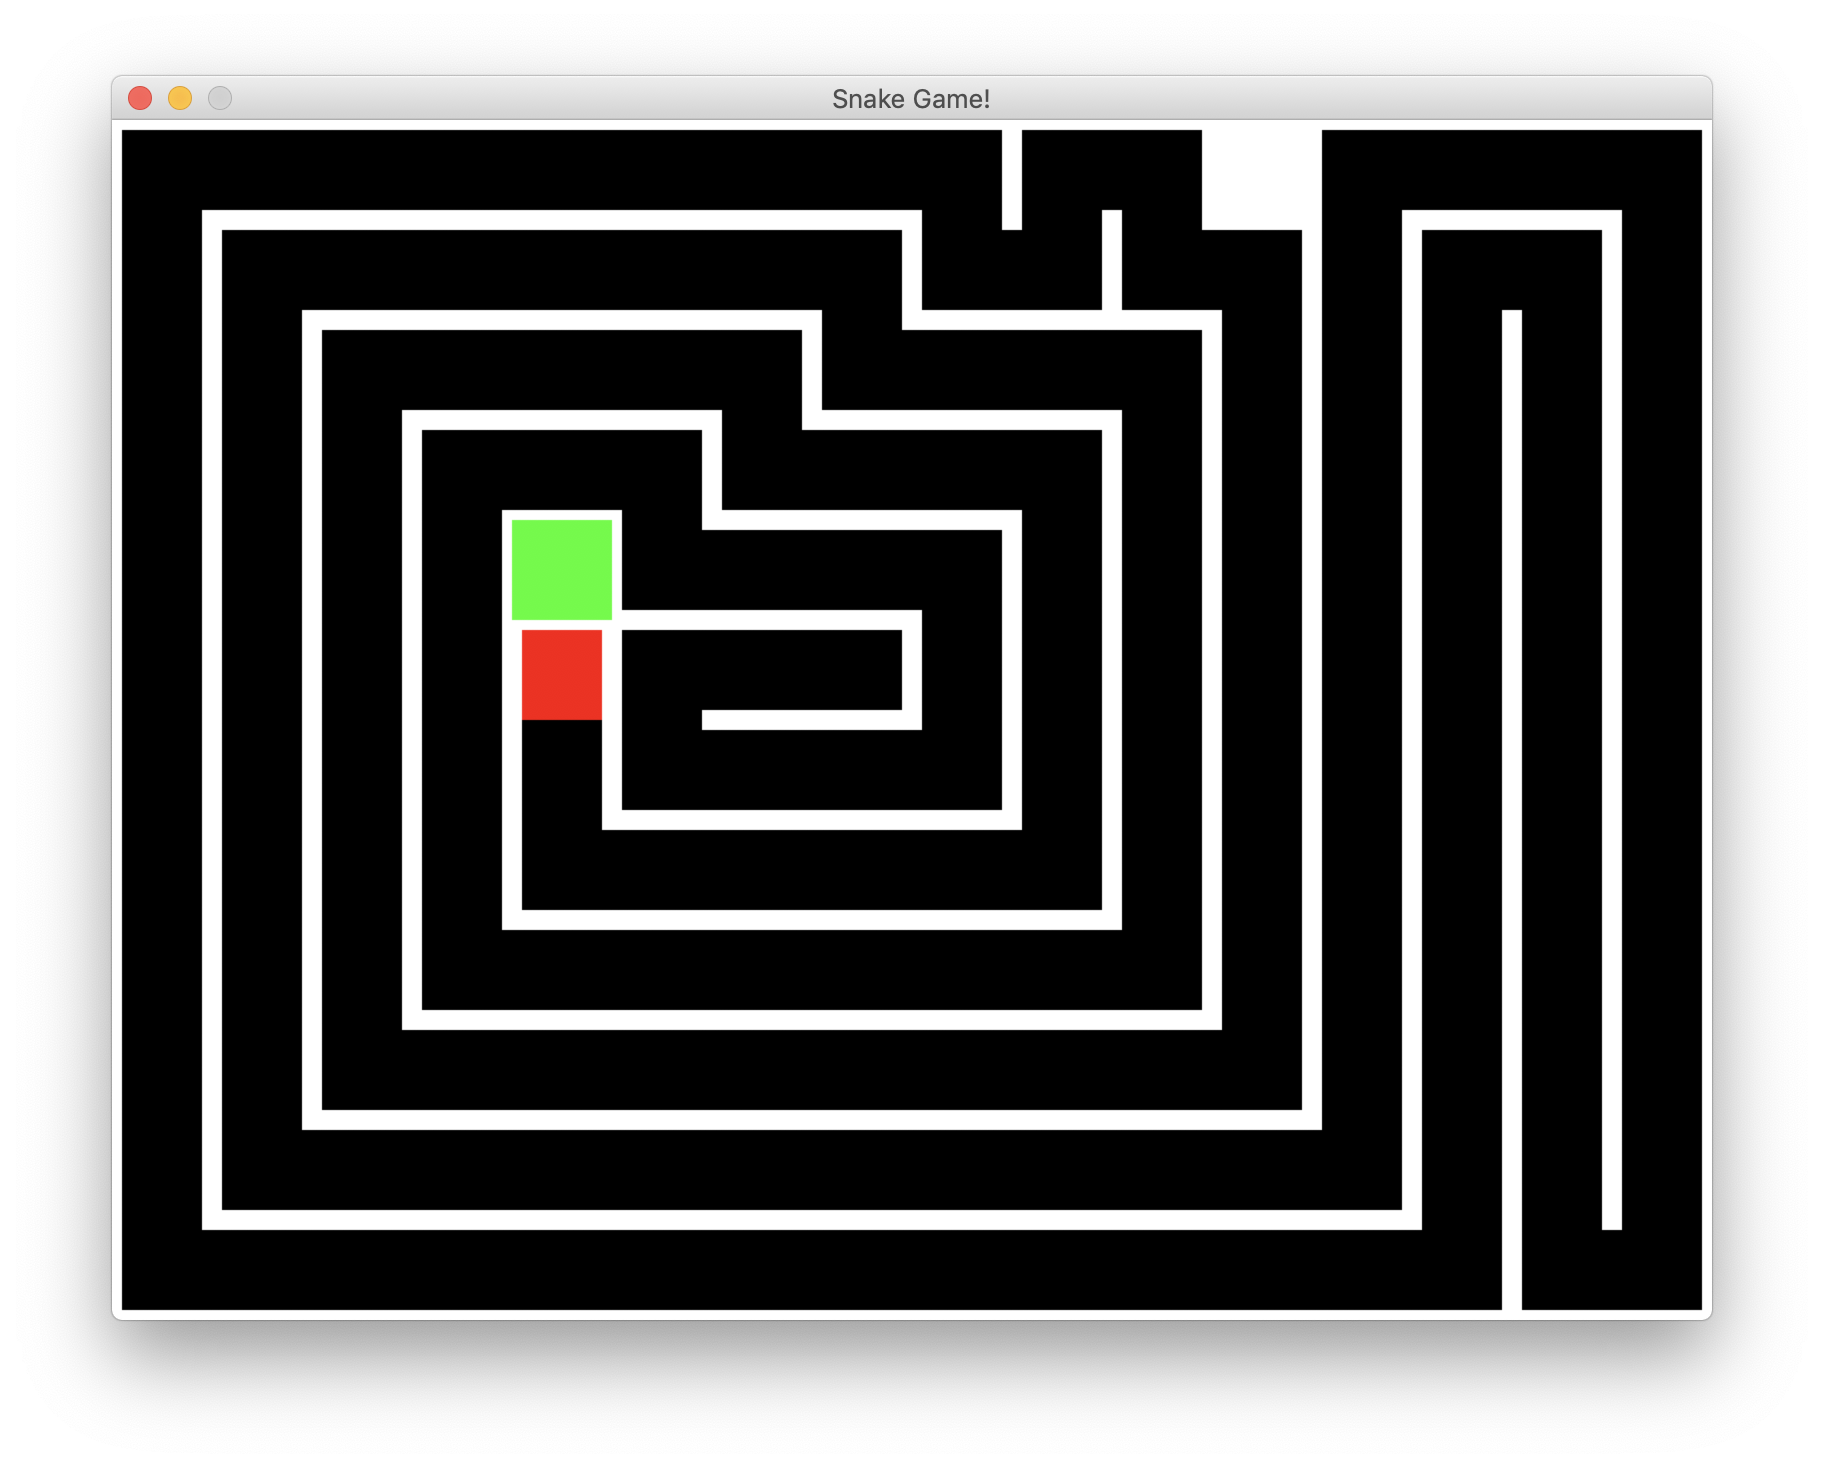
\includegraphics[width=\linewidth]{assets/lp5.png}
% \caption{caption} \label{fig:label}
\end{minipage}
    \caption{最长路近似算法取得最优解(图为从蛇头到蛇尾的最长路)} \label{fig:lp}
\end{figure}

\subsection{算法实现}
最长路近似算法的算法实现如\autoref{lst:longest}所示。代码仅展示重要部分。\\

设变量sp存储的是最短路的走法中每一步的方向。算法一开始初始化idx为0,
cur为最短路的第idx步的坐标。该算法反复尝试拓展第idx步,以求将第idx步
拓展为$i_0, i_1, i_2$三步。其中$i_1$步就是第idx步,$i_0$和$i_2$是
额外拓展的两步,这两步走的是相反的方向(例如上和下,左和右)。如此一来,
$[i_0, i_1, i_2]$三步的效果完全和$[idx]$步的效果一致。\\

举个例子,例如最短路中第idx步是向上走的。拓展算法会尝试把[UP]拓展为
[LEFT, UP, RIGHT](分别对应$i_0, i_1, i_2$)。可以看到,$i_1$等于
第idx步的走向。$i_0$和$i_1$是两个相反的方向,且与第idx步\emph{垂直}。\\

以上的描述解释了\autoref{lst:longest}注释(1)处代码的作用。它使用
insert方法,分别做insert(idx, *) 和insert(idx + 2, *),以完成以上描述
中的拓展。\\

\emph{NOTE:在拓展之后,最短路的第idx步的方向发生了变化。但第idx步时所在
的坐标不变}\\

\emph{NOTE:算法会在最短路的0$\sim$idx段完全拓展完毕后,再自增idx,尝试拓展
idx+1段}。
\begin{figure}[!hbt]
\begin{itemize}
\item[] \begin{lstlisting}[style=mypython, label=lst:longest, caption=最长路算法的实现]
def longest_path(self, target):
    '''
    @variable sp 最长路列表
    '''
    # idx如正文描述
    idx = 0
    # 最短路的第idx步时的蛇头位置
    cur = self.snake.head()
    while True:
        extended = False
        direction = sp[idx] # 最短路的第idx步的走向
        if direction in ['U', 'D']:
            test_extend = ['L', 'R'] # 可能的拓展方向
        else:
            assert(direction in ['L', 'R'])
            test_extend = ['U', 'D']
        # next_cur 是 cur 沿着最短路走一步得到的结点 
        next_cur = self.pos_move(cur[0], cur[1], direction)
        for d in test_extend: # d是可能的拓展方向
            # t1 和 t2分别是cur和next_cur朝着方向d移动一步得到的结点
            t1 = self.pos_move(cur[0], cur[1], d)
            t2 = self.pos_move(next_cur[0], next_cur[1], d)
            # 如果t1和t2结点是能拓展的(该块在地图区域内且该块没有被占用)
            if self.__exstendable(*t1, game_map) 
                and self.__exstendable(*t2, game_map):
                extended = True
                # (1)
                sp.insert(idx, d)
                sp.insert(idx + 2, self.rev_map[d])
                # 将t1和t2的所在块设置为占用
                x, y = t1
                game_map[y][x] = 'X'
                x, y = t2
                game_map[y][x] = 'X'
                break
        # 最短路从0到idx这一段已经完全无法拓展了。将idx加1
        if not extended:
            cur = next_cur
            idx += 1
            if idx >= len(sp):
                break
    return True, sp
\end{lstlisting}
\end{itemize}
\end{figure}

\subsection{最短路算法}
本项目采用广度优先搜索算法寻找最短路。事实上,可以将该算法替换成
A Star算法,获得更多性能的提升。

\section{效果评价}\label{sec:eval}
贪吃蛇寻路算法的最终结果如\autoref{fig:finish}所示。\\

其中红色方块是蛇头(右上角)。绿色方块是水果(中间)。黑色方块是
蛇身。白色方块是蛇身未占领的区域。\\

从\autoref{fig:finish}可以看到,贪吃蛇几乎占满了全部的地图区域。
此时由于蛇没有处于图的哈密顿回路上,故蛇永远都无法吃到那个绿的水果。此时可以认为游戏结束,
算法完美地完成了它的任务。
\begin{figure}[!hbt]
    \begin{center}
    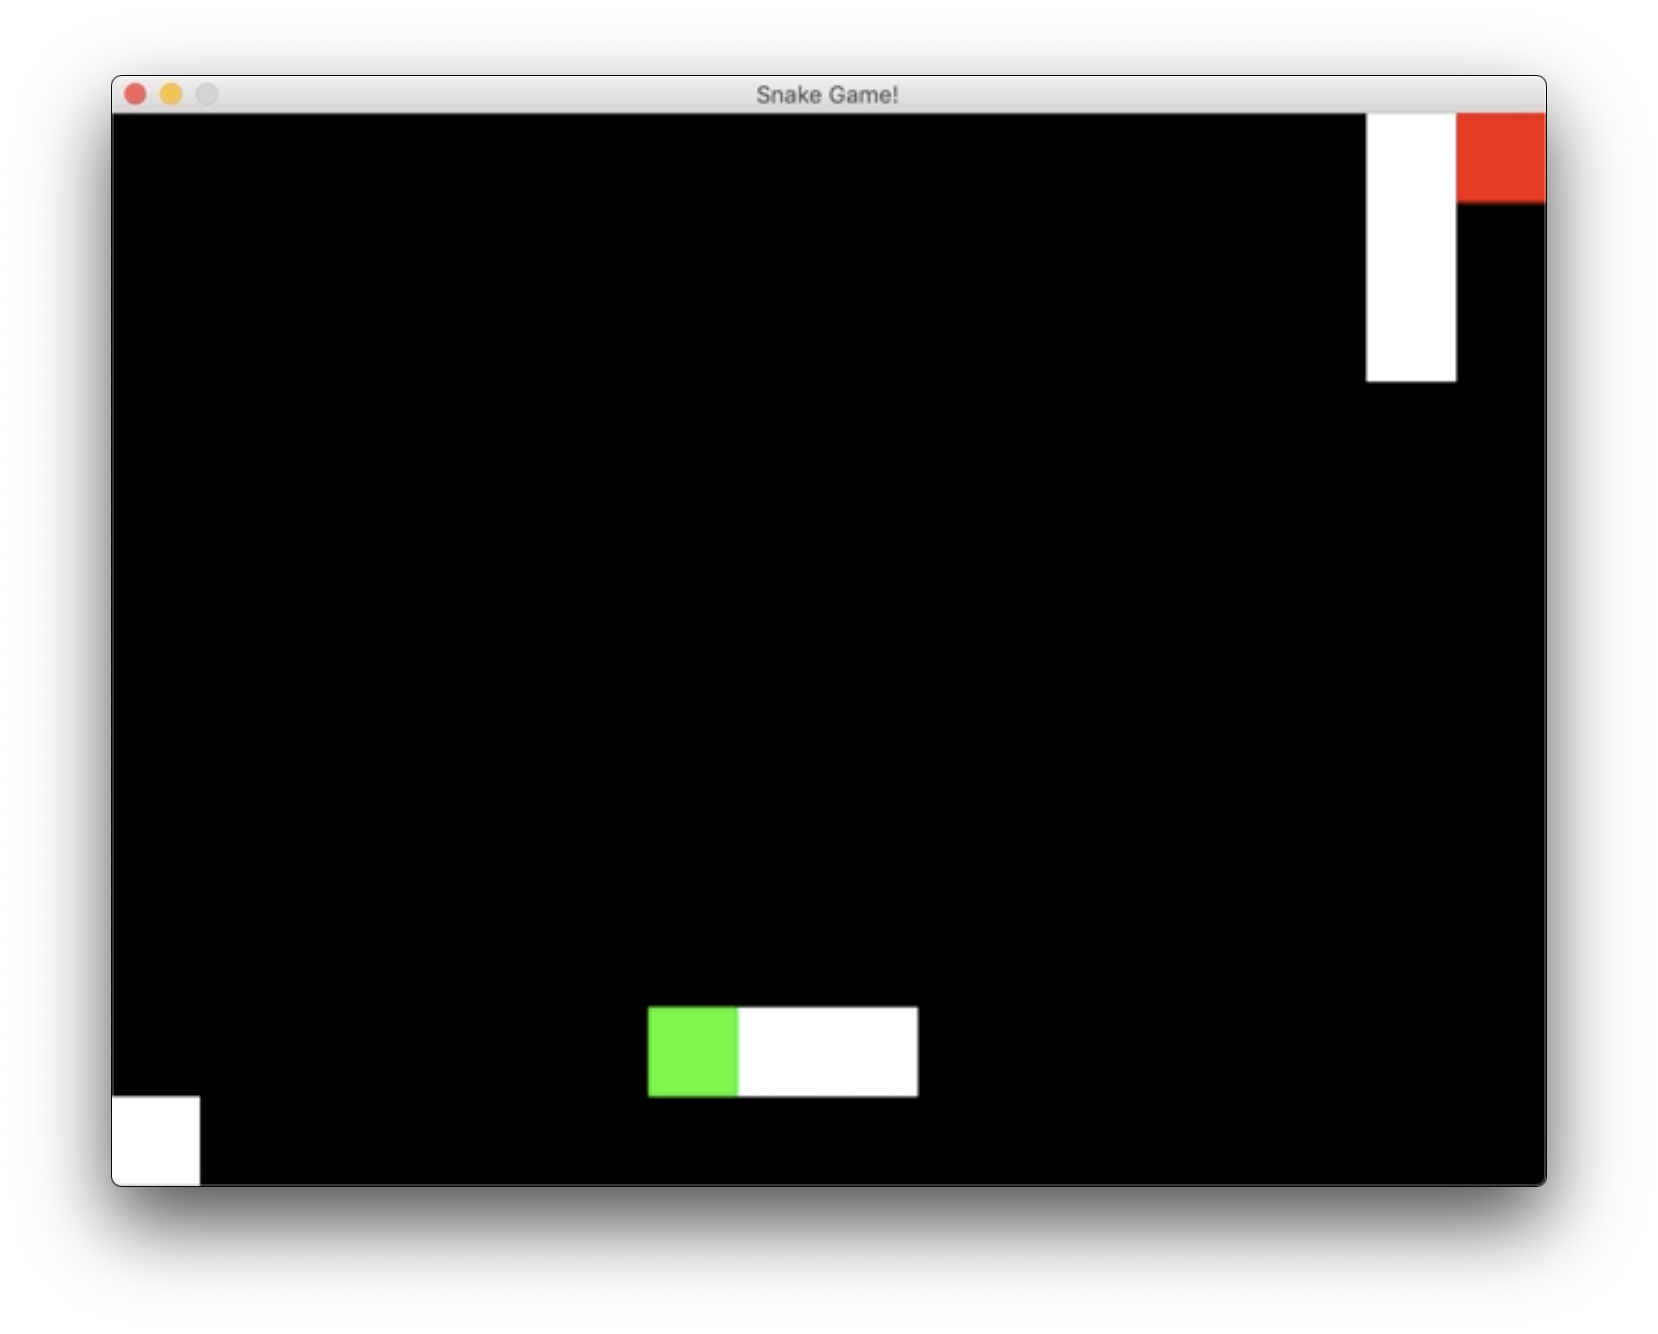
\includegraphics[scale=0.4]{assets/finish.png}
    \caption{贪吃蛇算法的最终场景\label{fig:finish}} 
    \end{center} 
\end{figure} 

\section{实验总结}
% \begin{appendices}
% \section{参考文献} \label{sec:reference}
% \section{伪代码补充} \label{sec:file}

% \end{appendices}
\end{document}
